\chapter{BoDMaS: Bio-Inspired Algorithm to Detect and Counteract Selfishness}\label{Chap6}
\echapter{BoDMaS: Bio-Inspired Algorithm to Detect and Counteract Selfishness}

\section{Introduction}\label{Chap6_01}
\esection{Introduction}
Emerging socially-aware networks that leverage social behaviors of participating users to improve networking throughput is gradually dominating wireless communication towards replacing traditional wireless networks. Among various socially-aware networks, ASNETs are gaining momentous ground due to their unique characteristics, particularly low resource consumption cost, mobility support, and infrastructure-less settings. Such features are often observed in biological processes that inspire inventing and designing novel cooperative architectural concepts~\cite{SBalasubramaniam2011}. ASNETs are proliferating as the common communication platform in broadly important areas such as pervasive conference/meetings and health-care, remote environmental monitoring and public safety, and ubiquitous urban data acquisition and national defense.

In socially-aware networking environments, users generate large amounts of data by exploiting capability-rich mobile devices which are willing to share their capabilities with users through social relationships, social ties or greater similar interests. However, successful adoption of ASNET services (e.g., data dissemination and replication), is inhibited in the absence of motivation/incentive for participating users who collaborate and share their resources. Cooperation among users is crucial to the survival of the network, as it forms the basis for key network services. If  users (selfish users) refuse to collaborate in delivering the network services, end-to-end connection may not be possible leading to network performance degradation. Existing solutions assume that users are willing to collaborate with others \cite{MEirinaki2014}. However, users in practice are selfish with varied degrees of selfishness (from non-selfish to fully-selfish) depending on the strength of their social-tie with the underlying network, especially when there is no cooperating motivation/incentive \cite{QLi2010}. Selfish users are unwilling to spend their precious resources for operations that do not directly benefit them~\cite{KGopalakrishnan2009}. For example, they may be willing to collaborate with socially-tied users (e.g., friends, co-workers, room-mates), but not others. Fig. 6.1 shows an example of a selfish user who inhibits efficient data forwarding in an exemplary scenario. The sender user $S$ has two route choices ($S\rightarrow A\rightarrow B \rightarrow R$ and $S\rightarrow A \rightarrow C\rightarrow D\rightarrow R$) to forward data to the user $R$ at the receiver side; one is 3-hop and another 4-hop far from receiver. Though efficient networking demands data transmission through lower-hop route (3-hop in this example), the selfish user $B$ located in middle of 3-hop route inhibiting data transmission via this route. Hence, transmission must be carried out via longer route over 4 hops leading to higher communication overhead \cite{SAbolfazli2014}. Therefore, it is essential to detect selfish users and isolate them to limit their negative behavioral impact on the network performance.
\begin{figure}[t]
\begin{center}
  \begin{tabular}{c}
  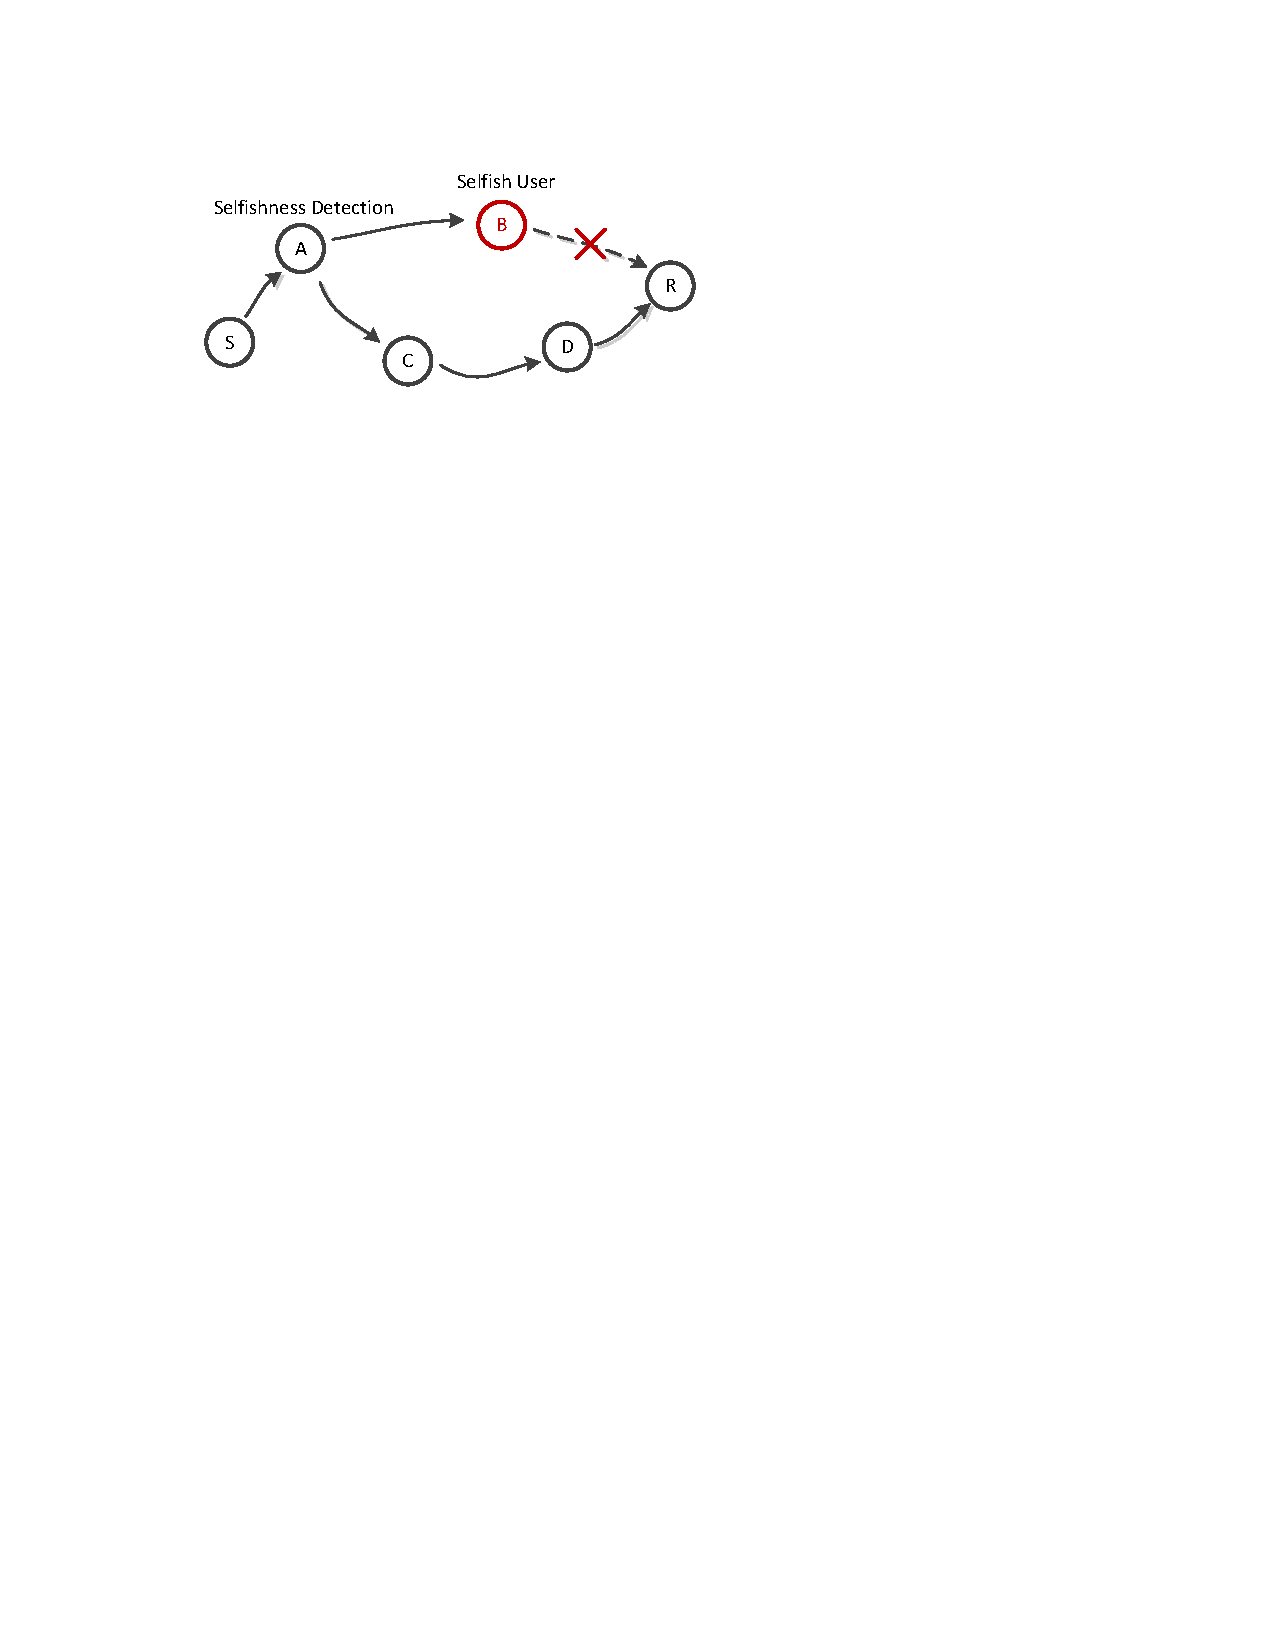
\includegraphics[width=0.5\textwidth]{Chap6-Fig1.pdf}
  \end{tabular}
  \caption{An example demonstrating user selfishness in forwarding data from source to destination.}
\end{center}
\end{figure}

Although a variety of solutions aim to address the problem of detecting and isolating misbehaving users in wireless networks~\cite{JChoi2011}, most existing works have focused on addressing selfishness by employing approaches such as reputation \& incentive based~\cite{MTRefaei2010}, trust-based~\cite{UVenkanna2013}, ACK-based~\cite{NKang2010}, game-theory~\cite{KAkkarajitsakul2013} or quorum-based~\cite{EMannes2012} mechanisms to incentivize and motivate users to collaborate in services for others. In spite of significant findings in the detection and isolation of users' selfishness, there are still numerous issues that limit their applicability~\cite{SDjahel2011}. Firstly, social behaviors of participating nodes are neglected in design and development of existing algorithms and hence makes them inefficient to be directly applied to ASNETs to deal with selfishness. Secondly, a huge overhead is induced from sharing reputation information amongst the users, additional acknowledgment packets dissemination, and decision ambiguity that arises if the requested user refuses to return an acknowledgment. Thirdly, cooperative users might be indirectly punished due to their location in the network. Fourthly, network might be flooded by when a user sends the same data several times to the same receiver. Lastly, existing bio-inspired solutions (such as~\cite{EMannes2012}) in this field of research consider only quorum systems without social behavior consideration such as social ties.

ASNETs lack a centralized controlling and monitoring terminal, thus, making it a challenging task to  effectively detect and isolate such misbehaving nodes from the network. Selfishness is a non-cooperative act of misbehavior, which is notably different from malicious behavior. It is noteworthy that our focus in this chapter is only on selfishness and thus we ignore malicious behaviors. To overcome the above limitations of existing algorithms, we design a bio-inspired algorithm named BoDMaS aiming to detect and counteract selfishness in ASNETs where high cooperation is highly desirable. We develop our work taking inspiration from a biological mechanism resident in bacteria (quorum sensing) and social community systems. Our initial results are extremely encouraging, indicating that the choice of social behavior is critical and that novel techniques can be successfully imported from biologically inspired models.

In this chapter, we are mainly focusing on user's behavior with respect to data replication operations (i.e., query/update) at the top of the data management model. Under this focus, each user can be classified as either cooperative (well-behaving) or selfish (misbehaving). This model may also apply to malicious users indirectly to some extent when it comes to timeout manipulations. However, malicious behavior is not to be under-estimated and shall undoubtedly be considered in our future work. Other classes of reliability model (trust and adversary) are also outside the scope of this chapter. The remainder of this chapter is structured as follows. \ref{Chap6_02} reviews related works in the literature. \ref{Chap6_03} presents an overview of the system model and assumptions. \ref{Chap6_04} provides the detailed design architecture and briefly describes the functions of each BoDMaS component. Section~\ref{Chap6_05} demonstrates the effectiveness of our proposed system and discusses the results. The last section formalizes the conclusion from the work conducted.

\section{Related Work}\label{Chap6_02}
\esection{Related Work}
There are several research works that have applied the above mentioned approaches. Gera {\it et al.}~\cite{PGera2011} proposed an opinion-based cooperative trust model in the presence of malicious nodes. With respect to the behavior observed, each node determines the trustworthiness of the other nodes. Their trust model exploits information sharing among nodes to accelerate the convergence of trust establishment procedures, and is further robust against the propagation of false trust information by malicious nodes. However, continuous information sharing overhead is degrading native resources of wireless nodes in the network. The authors in~\cite{DHales2005} focus on the problem of maintaining significant levels of cooperation in peer-to-peer networks. Their algorithm is adapted from novel "tag" models of cooperation that do not rely on explicit reciprocity, reputation or trust approaches. Another line of work by Li and Cao~\cite{QLi2012} uses contact records based on which the next contacted node can detect if the node has dropped any packet in order to develop a distributed scheme to detect selfishness in DTNs. The same authors of~\cite{QLi2012} have published a scheme named SSAR (Social Selfishness Aware Routing) ~\cite{QLi2010}, which considers both users' willingness to forward and their contact opportunity to select a forwarding node, resulting in a better forwarding strategy than those based solely on contact. However, in non of these works, focus is given to the selfish attitude of nodes and researchers are trying to motivate cooperation among nodes.

McCoy {\it et al.}~\cite{DMcCoy2007} presented MIND, a reputation-based authentication protocol for identifying and handling misbehaving and malicious users in the neighborhood. In this protocol, each user conducts a continuous follow-up over its neighbor user's forwarding behavior by comparing the incoming and outgoing data of its neighbor. However, this can cause a higher detection rate for false positives. Furthermore, when a user queries its neighbors and if the reply is invalid or fails to reply, the user decides that a neighbor has failed without giving any reason for the failure. In addition to the reputation-based mechanisms, there are some proposals on enforcing collaboration for wireless ad-hoc networks (i.e.,~\cite{NJiang2007}), addressing the problem of resilience in the network with the presence of misbehaving users (i.e.,~\cite{HJLeBlanc2013}) and blacklisting misbehaving users while maintaining the privacy in the network (i.e.,~\cite{PPTsang2011}).

LeBlanc {\it et al.}~\cite{HJLeBlanc2013} showed that users' connection or neighborhood is no longer adequate for the assurance of resilient consensus when the users use their own inbuilt nature that only require each user to know its own neighborhood. However, the results in their proposal apply to directed graphs and consider undirected graphs as an exceptional case. In addition to that, they categorize misbehaving users as a restricted type of Byzantine user in which every user is required to send similar message to all of its neighbors which causes the users to consume high energy.  On the other hand, Nymble~\cite{PPTsang2011} has been proposed with the aim of permitting anonymous blacklisting of misbehaving users. This proposal tries to reinvent the common practice of address banning, without actually telling a user's address. However, this protocol exposed to some sensitive security and trust issues reducing from the usage of trusted third parties that can simply work together to disrupt a user's secrecy.

From Komali {\it et al.}'s~\cite{RSKomali2008} and Pelechrinis {\it et al.}'s~\cite{KPelechrinis2012} perspective, it is difficult to justify the cooperative theory because nodes are either competing for network resources or conserving their own limited resources. Therefore, they proposed an algorithm called DIA($\delta$-Improvement Algorithm) in which each node makes some decrements in its power level if the change improves its operation. However, their performance evaluation shows that there might be a fundamental conflict between an efficient and fair allocation. It shows that it is important to integrate load balancing and fairness mechanisms to misbehavior detection mechanisms, to predict how much the user is willing to offer his resources to strangers under a probabilistic framework and assign other utilities mechanism. However, these algorithms are unable to fulfill unique requirements of ASNETs.

Data management, particularly data availability is one of the most crucial tasks in ASNET environments. Replication is one of the prominent techniques for ensuring the accessibility of data among partitioned communities. Data replication is a technique of creating and managing replica. Replica is a data item that is stored redundantly at multiple communities. In chapter~\ref{Chap4}, we proposed ComPAS which detailed the means of allocating replicas in different communities in order to increase data availability. However, one of the assumptions in designing the system model is that all the participating users are cooperative in every aspect, such as forwarding read queries and update operations which is not the reality in ASNETs. In order to address challenges emerging from misbehaving users in replication operations for MANETs, Mannes {\it et al.}~\cite{EMannes2012} proposed $QS^2$ by incorporating bio-inspired mechanisms into quorum systems. Quorum systems are powerful mathematical tools to reason about distributed implementations of shared objects including read/write operations~\cite{JLuo2003}. In particular, quorum systems have been used for reasoning in implementations that tolerate misbehavior and are optimally resilient to process failures. More sophisticated forms of quorum systems have been introduced to cope with different failures and these require larger intersections among quorums, eventually leading to an increased overhead.

Drawing from the analogy with existing quorum systems as communities, we believe that applying biologically inspired mechanisms~\cite{SBalasubramaniam2011} in this regard will help to reduce the limitations of existing algorithms. This has also been proved in the work from our lab~\cite{FXia2014} related to data forwarding for socially-aware networks. To the best of our knowledge, BoDMas is the first work to consider social willingness in designing a bio-inspired algorithm to detect and neutralize the impacts of selfish users within dynamically changing network conditions of ASNETs.

\section{Models and Assumptions}\label{Chap6_03}
\esection{Models and Assumptions}
In this section, we first present the overall model of a simplified ASNET system illustrated in Fig. 6.2 and explain inter-layers interactions and functionality of its major components. Subsequently, we discuss matching analogy between bacteria operation and ASNET functionality. Network model (including social graph and user mobility components), data management model (consisting of replication and load balancing components), and reliability model (comprising attack, trust, and adversary components) are described. The successful operation of ASNETs entirely depends on the cooperation among sub-models and components. For scalability and resilience reasons the current system model needs to be redesigned.

\begin{figure}[t]
\begin{center}
  \begin{tabular}{c}
  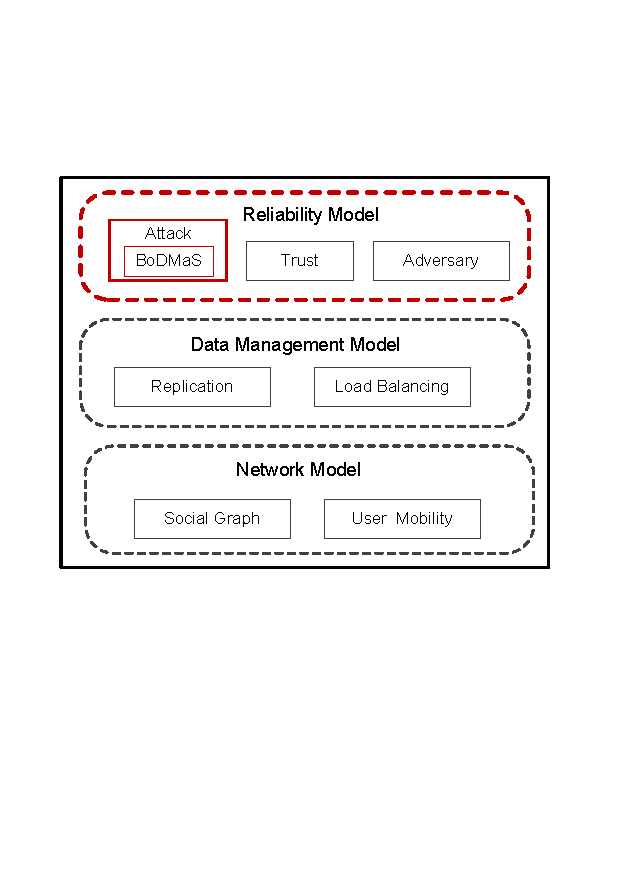
\includegraphics[width=0.55\textwidth]{Chap6-Fig2.pdf}
  \end{tabular}
  \caption{Simplified ASNET Middleware System Model.}
\end{center}
\end{figure}

\subsection{Network Model}\label{Chap6_03_01}
\esubsection{Network Model}
Network in ASNET is modeled using social graph and user mobility. Social networks exhibit the small world phenomenon that node encounters are sufficient to build a connected relationship graph~\cite{FXia2013}. Such a graph is an abstract graph where vertices represent individual people and edges describe social ties between individuals. Through the use of a social graph, a variety of social metrics (e.g. social relationship, communality, centrality, and similarity) can be easily calculated. Therefore, it is crucial to obtain social graphs for social-based data management design approaches like ASNETs.

We model the social community network as a bidirectional, weighted communication that is symmetrical at every link between users. It means that if a user $Y$ is able to receive a message from user $X$ at time $t$ then user $X$ can also receive a message from user $Y$ at time $t$. As in other studies~\cite{QLi2010}, \cite{KGopalakrishnan2009}, this assumption is often valid using selected wireless MAC layer protocols (i.e. IEEE 802.11) requires bidirectional communication for reliable transmission. The network is composed of a vertex set $G$ of all $n$ users/nodes identified by $\{d_0, d_1 ... d_{n-1}, d_n\}$, and a set of edges, $E$, to be the social links between users. Every user $d_i \in G$ has a unique address or identification and the same processor and energy capacity. The weight of edge $XY$ is $X$'s willingness to forward query/update packets for $Y$. The weight of edge $XY$ and that of $YX$ may be different. In ASNETs, users have limited bandwidth and computational capability. Furthermore, users are assumed to rely on intermediate users to route packets since they may not reach directly due to their coverage area~\cite{HBLiaqat2014}.
\begin{figure}[h]
\begin{center}
  \begin{tabular}{c}
  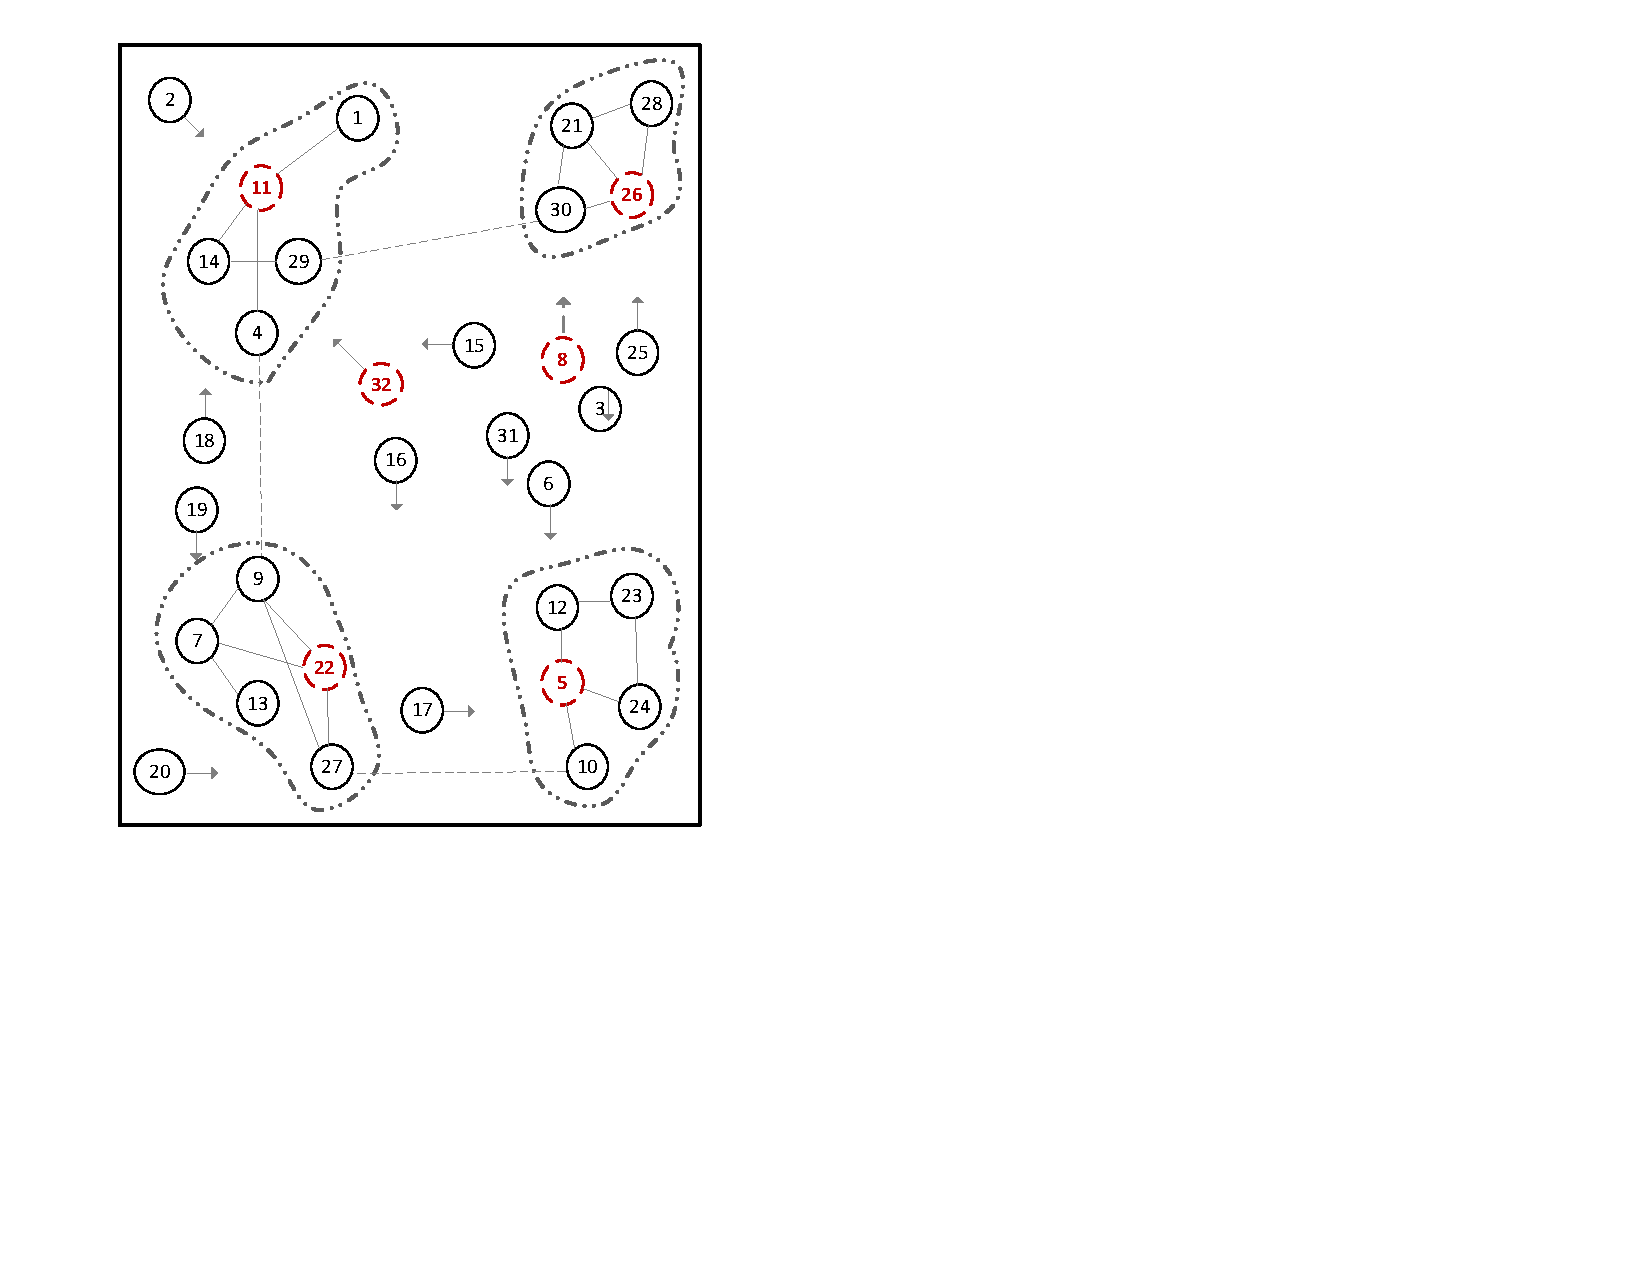
\includegraphics[width=0.55\textwidth]{Chap6-Fig3.pdf}
  \end{tabular}
  \caption{Illustration of user mobility within an ASNET of 32 users. There are four communities (denoted using the gray dotted lines) and 32 mobile users(denoted using circles), where some users are selfish (represented by the red dashed circles) and some are roaming outside a community (moving directions are represented using arrows).}
\end{center}
\end{figure}

User mobility is another component in modeling ASNET networks. Users move according to the group movement pattern in a surrounded area. Community partitions in the network can occur when the network between the communities fail simultaneously due to movement of users or scarce resources. Group mobility refers to the scenario where several mobile users tend to move together. The system tries to solve the problem of selfishness in replication operations by exploring group mobility. The underlying group mobility model is assumed to be RPGM as used in chapter~\ref{Chap4} of this dissertation. In our system, each mobile user first exchanges its motion behavior with its neighbor based on the social relationship in the community. Mobile users may collaborate and, hence, move as a group instead of independently. RPGM is a better choice to model this kind of team collaboration behavior. As shown in Fig. 6.3, all users are divided into several mobility groups and all mobile users within the same mobility group are of similar moving behavior~\cite{AMAhmed2014}.

\subsection{Data Management Model}\label{Chap6_03_02}
\esubsection{Data Management Model}
In ASNETs, replication helps to avoid data losses in case of an unpredictable group mobility that causes community partition and also aids in reducing the number of hops when a data is transmitted. This work employs ComPAS (Chapter \ref{Chap4}) as the data management (replication) model. Note that, other schemes could be applied, nevertheless, ComPAS was chosen because it can significantly improve ASNETs performance by exploiting social relationship while replicating in the community to achieve better efficiency and consistency which makes it more appropriate. Further, it can also reduce the query delay, since users can get the data replicas from some nearby communities. By replicating, data availability can be improved because there are multiple replicas in the network and the probability of finding one copy of the data is high~\cite{ADerhab2009}. {\it Replica} is a data item that is stored redundantly at multiple communities. We define data replication as a technique of creating and managing duplicate versions of data items. Users comprise of performing two types of operations: {\it query} and {\it update}.

Simply, ComPAS is a system based on partitioning of social community combined with social relationship and a user level replication so that data availability for all users is guaranteed. The system gives a fixed number of replicas required for each user that results in an efficient replication solution. It is based on a perception that if we need to place a replica copy for a user $i$ somewhere, the most desirable location should be the primary storage place of most neighbors of $i$; this way, most neighbors will benefit from this replica when they issue a read query. Furthermore, it aims to find an efficient and consistent way to store $X$ replicas for each user's data in the storage space at $Y$ communities $(X < Y)$ and it choose the value of $X$ depending on the replication budget of the system and its desired availability. For detailed illustration of ComPAS's operation, refer to Chapter \ref{Chap4}.

\subsection{Reliability Model}\label{Chap6_03_03}
\esubsection{Reliability Model}
Reliability in ASNET can be verified from a different perspective. Our way of understanding categorizes it as attack, trust and adversary components.  As mentioned in the previous sections, among the components our focus is only on the {\it attack component (selfishness)}. Selfish users work in the network for their own benefit. They simply do not cooperate with other users in data transmission process to conserve their own energy, or give priority to their own interest. These selfish users disturb the performance of ASNET to a great extent. {\it Trust} is a critical determinant of sharing information and developing new relationships in a network~\cite{YNajaflou}. Although trust is not our target and it is not essential to our proposed scheme, we assume the source of data is anonymous to intermediate users. Other technical aspects related to trust such as authentication is out of the scope of this dissertation. Malicious attacks (i.e. modifying or injecting malicious data in the replication system) and free-riding behaviors are grouped in {\it adversary component} and not our focus.

\subsection{Ad-hoc Social Network and Bacteria Analogy Matching}\label{Chap6_03_04}
\esubsection{Ad-hoc Social Network and Bacteria Analogy Matching}
In biological systems, two main entities can be observed~\cite{JLFernandez-Marquez2013}, namely (1) the organism that collaborates in the biological process (e.g., virus, ants, bees, fish, and bacteria) and (2) the environment (i.e., communities in ASNET). Among these, bacteria have complex social properties resulted from their communication abilities that govern their colony. These social behaviors enable the bacteria to evolve through various fluctuating environmental situations by utilizing cooperative and non-cooperative behaviors~\cite{MHasan2014}. They use quorum sensing to coordinate actions that cannot be carried out by a single bacterium. As individual and limited functionalities, their adjustment to the environment is very limited and therefore they rely on mobility. Quorum sensing can be defined as a decentralized coordination process which allows bacteria to estimate the density of their population and regulate their behavior accordingly by focusing on production and detection of chemical products called Acyl-Homoserine Lactone Autoinducers (AHL-Ai). Each bacterium is similar to a mobile node that extracts information from the environment, interprets the information, develops common knowledge and learns from past experiences~\cite{AEinolghozati2012}. Our proposed algorithm, considers social willingness as a social behavior and the characteristics observed in bacteria as a biological mechanism. AHL-Ai (hereafter $A_i$ for the sake of simplicity and brevity) acts as a signaling chemical gradient to detect and determine the amount of bacteria in the environment, allowing them to develop a collaborative behavior for the whole group, depending on the amount of bacteria engaged. The social behavior existence in both the community and bacteria makes a dynamic and autonomous solution, inspiring the proposed algorithm.
\begin{figure}[t]
\begin{center}
  \begin{tabular}{c}
  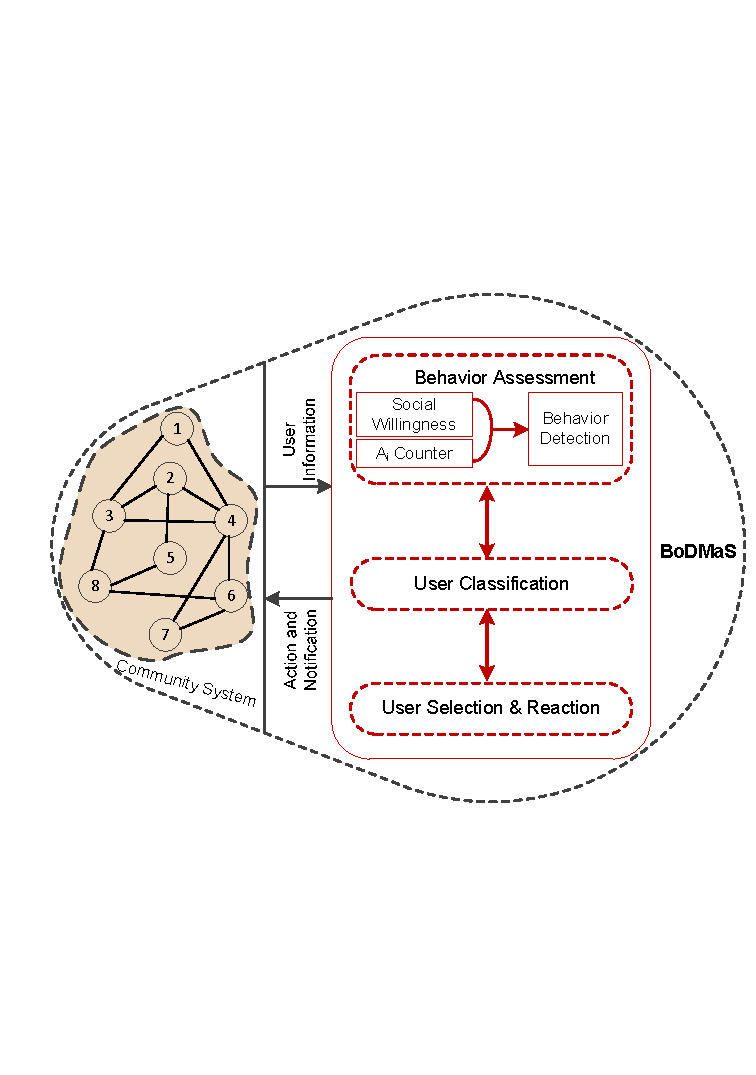
\includegraphics[width=0.65\textwidth]{Chap6-Fig4.pdf}
  \end{tabular}
  \caption{BoDMaS Architecture.}
\end{center}
\end{figure}

\section{Detailed Design}\label{Chap6_04}
\esection{Detailed Design}
Throughout this section, we present the overall architecture of our BoDMaS proposal and describe how BoDMaS fits into the typical ASNET system. We also describe functional interaction among BoDMaS components and provide algorithm pseudocode. We also discuss our model verification approach.

\subsection{BoDMaS Architecture}\label{Chap6_04_01}
\esubsection{BoDMaS Architecture}
BoDMaS aims to detect user's selfishness and counteract it to maintain the reliability of replicated data. Using three major components of behavior assessment, user classification, and user selection \& reaction, our proposal detects selfish users and takes actions against the involvement of selfish users in replication operations (i.e., query and update). The behavior assessment is executed by comparing social willingness level and observation of $A_i$ represented by the amount of replica updates, queries, and forwards issued by users. Fig. 6.4 present an illustrative view of our proposal consisting three basic components, namely: {\it behavior assessment}, {\it user classification} and {\it user selection \& reaction}.

Fig. 6.5 depicts interaction sequence among these major BoDMaS components. The behavior assessment component adopts and monitors social willingness level for intermediate users. Based on the score $A_i$ from the assessment, the next component evaluates the users in the process. The user classification component uses the score to compare it with the threshold ($Thr$) and identifies users with selfish behavior. Finally, the user selection \& reaction component selects cooperative users in order to perform data update and query operations, and takes action against selfishness by notifying other users. The remaining part of this section describes the details of each BoDMaS component.
\begin{figure}[t]
\begin{center}
  \begin{tabular}{c}
  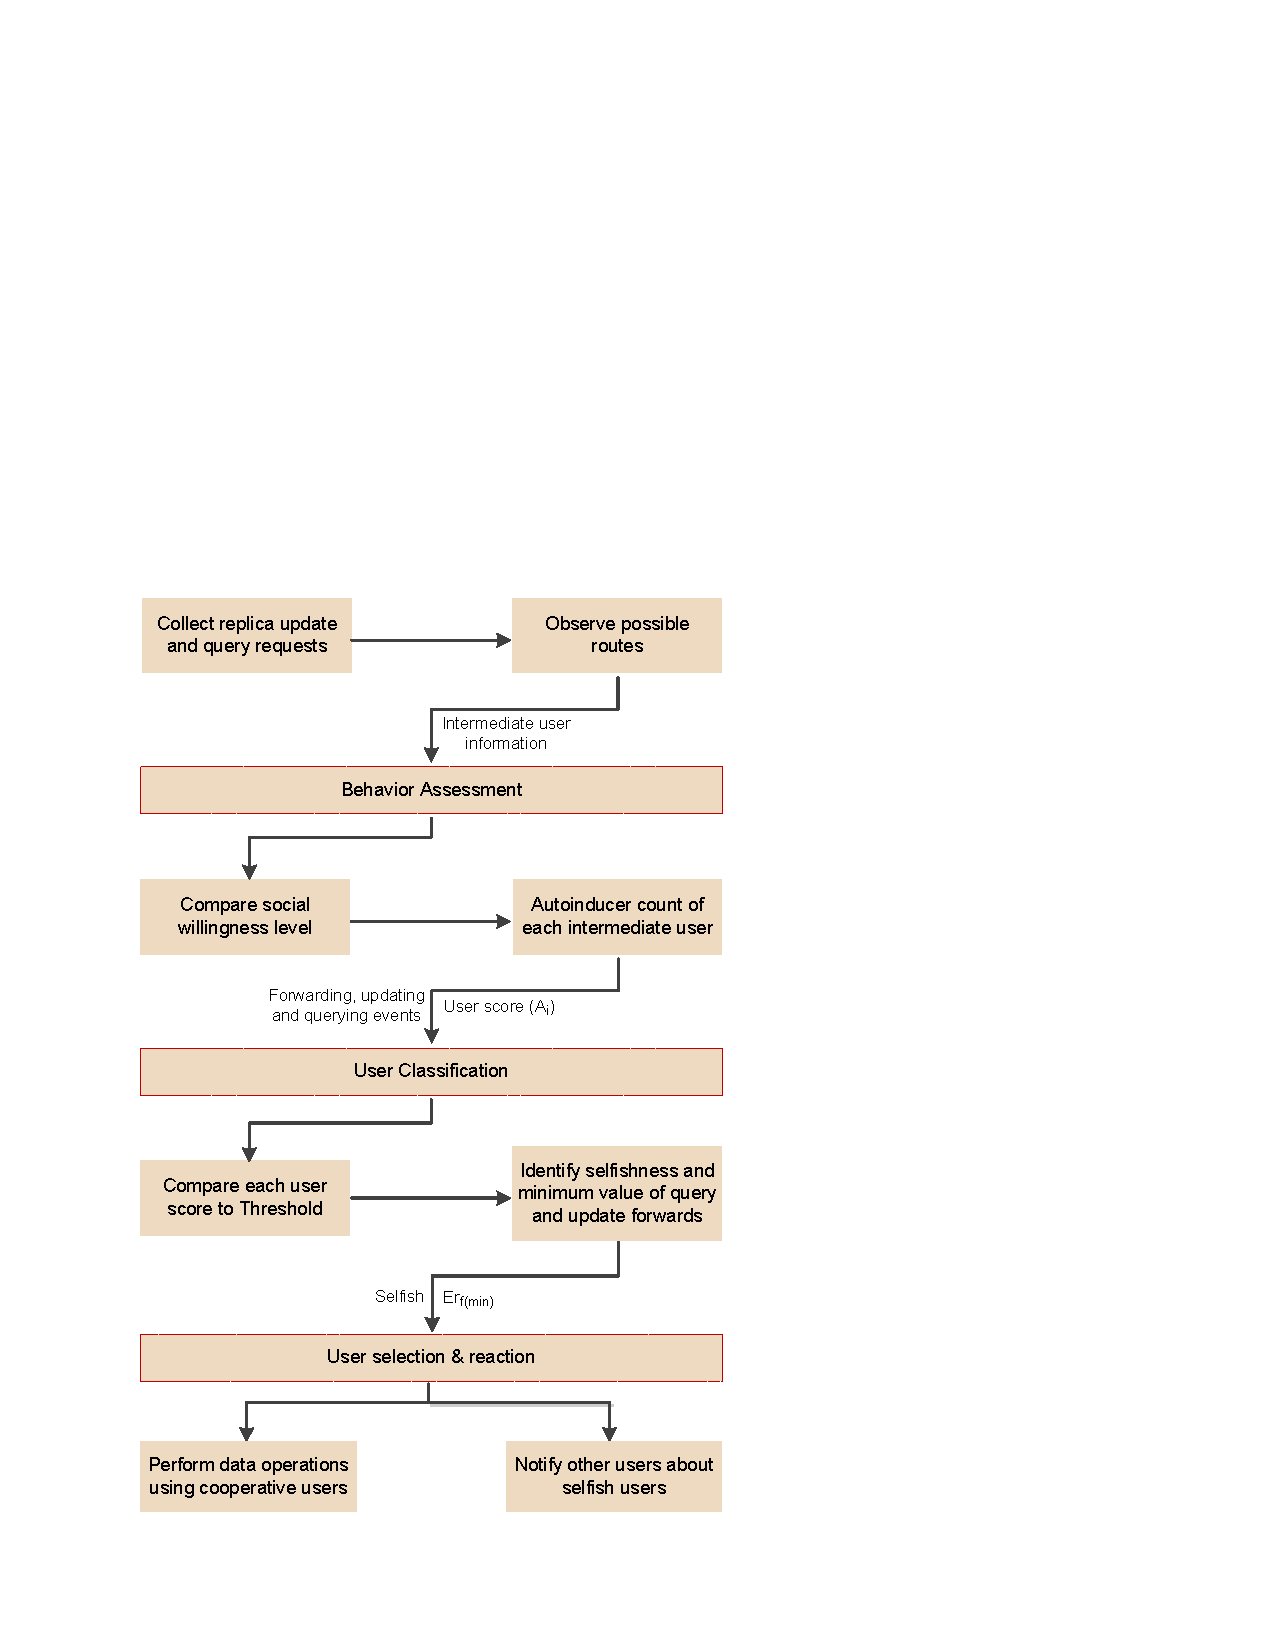
\includegraphics[width=0.6\textwidth]{Chap6-Fig5.pdf}
  \end{tabular}
  \caption{Functional interaction among BoDMaS components.}
\end{center}
\end{figure}

\subsection{Behavior Assessment}\label{Chap6_04_02}
\esubsection{Behavior Assessment}
To select an appropriate user for the operation, BoDMaS considers both users' willingness and $A_i$ counts. In our context, a social willingness means an interpersonal social tie between users that falls into the strong or weak range. A selfish user may demonstrate different behavior (cooperative) for users with strong social relationship. That is, the user is willing to provide better service to those with stronger ties than those with weaker ties, especially when there are resource constraints~\cite{QLi2010}. The work of Li {\it et al.}~\cite{HLi2012} presented three ways of assigning social willingness level: Uniform Distribution of Social Ties (UST), Clustered Distribution of Social Ties 1 (CST1) and Clustered Distribution of Social Ties 2 (CST2). Among these, we use UST that uniformly assigns random values between [0, 1] as willingness level ($\rho_{id}$) for the friendship between users.

The social willingness level between each pair of users $i$ and $d$ is characterized by a rational number $\rho_{id} \in$ [0, 1], where $\rho_{id}$ = 1 is strongest and $\rho_{id}$ = 0 means no willingness at all. Based on this value, the source user chooses the direct neighbor that has strong social tie as an input to the next step. High willingness level does not indicate that the user is not selfish, because there are cases in which the selected neighbor can hold or ignore the received data without doing the job (here is one of the importance of $A_i$ counter). To count replica forward operations $A_{i(f)}$, each user $i$ has $A_i$ counter linked with each neighbor having a social relationship in the community. The counting is conducted based on the communication between users, and occurs when a user receives replica query or update requests. Requesters attach their ID to the packet such that the behavior assessment component can use it to increment $A_{i(f)}$ counter for every user in the line (from source to destination).

\subsection{User Classification}\label{Chap6_04_03}
\esubsection{User Classification}
This component implements users' scores, assigned by the behavior assessment component (and possibly the sequence of operations that led to each score), to identify selfish users in the network. A common approach is to compare the user's score to the $Thr$ expected from a cooperative user. In order to get the correct $Thr$, the expected rate of forwards $Er_f$ according to the behavior of replication has to be estimated. This rate is calculated within a given period of time and used to set $A_{i(f)}$ threshold. A user that has $A_i$ count lower than this limit is classified as selfish.

\subsection{User Selection \& Reaction}\label{Chap6_04_04}
\esubsection{User Selection \& Reaction}
Finally, this component selects the cooperative users based on the score to perform the data operations. It also informs other users to avoid approaching selfish users. For example, in the case of update operations on replica, suppose that $Er_{f(min)}$ threshold is 3 forwards per second, a user whose score is greater than or equal to 3 is considered cooperative. Users with lower scores are classified as selfish. Algorithm \ref{alg:chap6_alg01} presents detailed BoDMaS operations.
\begin{algorithm}
\Begin{
    $\rho_{id} \leftarrow$ Social willingness level ($\rho_{id} \in$ [0, 1])\;
    $A_i \leftarrow$ Autoinducers count\;
    $A_{i(f)} \leftarrow$ Autoinducers count for replica forward\;
    $Thr \leftarrow$ Score expected from a cooperative user\;
    $Er_{f(min)} \leftarrow$ Minimum query and update forwards at time $t$\;
    {\bf Behavior assessment:}\\
     \For{all direct neighboring users}{
            compares $\rho_{id}$; where 1 is strongest and 0 is none;
            increment $A_{i(f)}$ counter for every user in the line (from source to destination);
     }
    {\bf User classification:}\\
            \For{all users' scores collected}{
            compare a user's score to a $Thr$\;
            \If{User $A_i$ count < $Thr$ limit}{
               classify the user as selfish\;
               $Er_{f(min)}$ value is identified\;
               }
    }
    {\bf User selection \& reaction:}\\
            take action against users according to their behavior\;
            \If{User score $\geq$ $Er_{f(min)}$}{
               user is considered cooperative\;
               perform data operations using cooperative users and notify other users about selfish users\;
               }
}
\caption{Pseudocode for BoDMaS}
\label{alg:chap6_alg01}
\end{algorithm}

To correctly verify the entire model, it is essential to calculate some values such as True Detection Rate ($TDR$) and False Detection Rate ($FDR$). Thus, we employ a set $M(b,r)$, containing all interactions of selfish users and a set $C(b,r)$ representing interactions of cooperative users in both query and update operations where $b$ represents the user class (either selfish or cooperative) after the detection result by BoDMaS and $r$ is the real class of that user. $TDR$ represents the amount of detected selfish users and it is calculated using Equation \ref{eq1}.
\begin{equation}\label{eq1}
TDR = \frac{\sum K_i}{|M|}  \hspace{1cm} \forall \hspace{0.4cm}i \in M,
\end{equation}
where $K_i$ = 1 if $b_i$ = $r_i$ and $K_i$ = 0 if $b_i \neq r_i$.

$FDR$ is of two types: False Negative ($FN$) and False Positive ($FP$). $FN$ detects the selfish users mistakenly classified as cooperative users. This is calculated using Equation \ref{eq2} with all the same $TDR$ assumptions.
\begin{equation}\label{eq2}
FN = \frac{\sum K_i}{|M|}\hspace{1cm} \forall \hspace{0.4cm}i \in M,
\end{equation}
where $K_i$ = 1 if $b_i \neq r_i$ and $K_i$ = 0 if $b_i$ = $r_i$. $FP$ measures the amount of cooperative users classified as selfish as shown in Equation \ref{eq3}, where $C$ denotes all the cooperative interactions. It's modeled as $C(b, r)$ where $r$ = 1 and 0 represents a selfish and cooperative users, respectively.
\begin{equation}\label{eq3}
FP = \frac{\sum K_i}{|C|}\hspace{1cm}\forall \hspace{0.4cm}i \in C,
\end{equation}
where $K_i$ = 1 if $b_i$ = $r_i$ and $K_i$ = 0 if $b_i \neq r_i$. The next section presents performance and efficiency evaluation results.

\section{Demonstration of Effectiveness}\label{Chap6_05}
\esection{Demonstration of Effectiveness}
\begin{table}
\centering
\caption{Simulation Parameters}
\renewcommand{\arraystretch}{1.5}
\begin{tabular}{|l|l|l|l|l|}
\hline
\multicolumn{1}{c}{Parameter} & \multicolumn{1}{c}{Value}\\
\hline
\multicolumn{1}{c}{Number of users} & \multicolumn{1}{c}{32}\\
\multicolumn{1}{c}{Number of communities} & \multicolumn{1}{c}{4} \\
\multicolumn{1}{c}{Defined area } & \multicolumn{1}{c}{400m X 400m} \\
\multicolumn{1}{c}{Users/community} & \multicolumn{1}{c}{$\approx$ 8}\\
\multicolumn{1}{c}{Number of simulations} & \multicolumn{1}{c}{10 trials}\\
\multicolumn{1}{c}{Simulation time} & \multicolumn{1}{c}{10 mins}\\
\multicolumn{1}{c}{User movement} & \multicolumn{1}{c}{RPGM}\\
\multicolumn{1}{c}{Maximum speed} & \multicolumn{1}{c}{2 - 20 m/s (variable)}\\
\multicolumn{1}{c}{Pause time} & \multicolumn{1}{c}{10s - 100s (variable)}\\
\multicolumn{1}{c}{Expected updating rate} & \multicolumn{1}{c}{$\lambda$ = 80}\\
\multicolumn{1}{c}{Expected querying rate} & \multicolumn{1}{c}{$\lambda$ = 24}\\
\multicolumn{1}{c}{Forward threshold} & \multicolumn{1}{c}{$Er_{f(min)}$ = 0.2 forwards per second}\\
\multicolumn{1}{c}{Number of selfish users} & \multicolumn{1}{c}{$N_{selfish}$ = 2, 4, 8 and 16 users}\\
\multicolumn{1}{c}{Confidence interval} & \multicolumn{1}{c}{95\%}\\
\hline
\end{tabular}
\end{table}
In this section, we present performance and efficiency evaluation of BoDMaS based on accessibility degree, detection rates, and network load balance. Results obtained by the evaluation of ComPAS integrating BoDMAS (represented by ComPAS$\uplus$BoDMaS) is compared to ComPAS without BoDMaS within the same scenarios. The scheme is analysed considering the presence of selfish users in ComPAS operations. The network is composed of 32 users within 4 communities, and users move according to RPGM into an area of 400$m^2$. The maximum speed range is 2-20 m/s with a varying pause time of 10s-100s. The expected updating and querying rates are $\lambda$=80 and $\lambda$=24, respectively. The forwarding threshold $Er_{f(min)}$ is 0.2 forwards per second. This scenario intends to represent an academic conference environment of mobile users that consists of different participants such as authors, organizers, speakers moving towards some common locations in the conference hall. The information shared concern about participants interest, like topics of presentations or key notes at multiple session rooms. Table 6.1 summarizes the detailed evaluation parameters we use for simulation to demonstrate the effectiveness of our algorithm.

\subsection{Accessibility Degree}\label{Chap6_05_01}
\esubsection{Accessibility Degree}
\begin{figure}[t]
\begin{center}
  \begin{tabular}{c}
  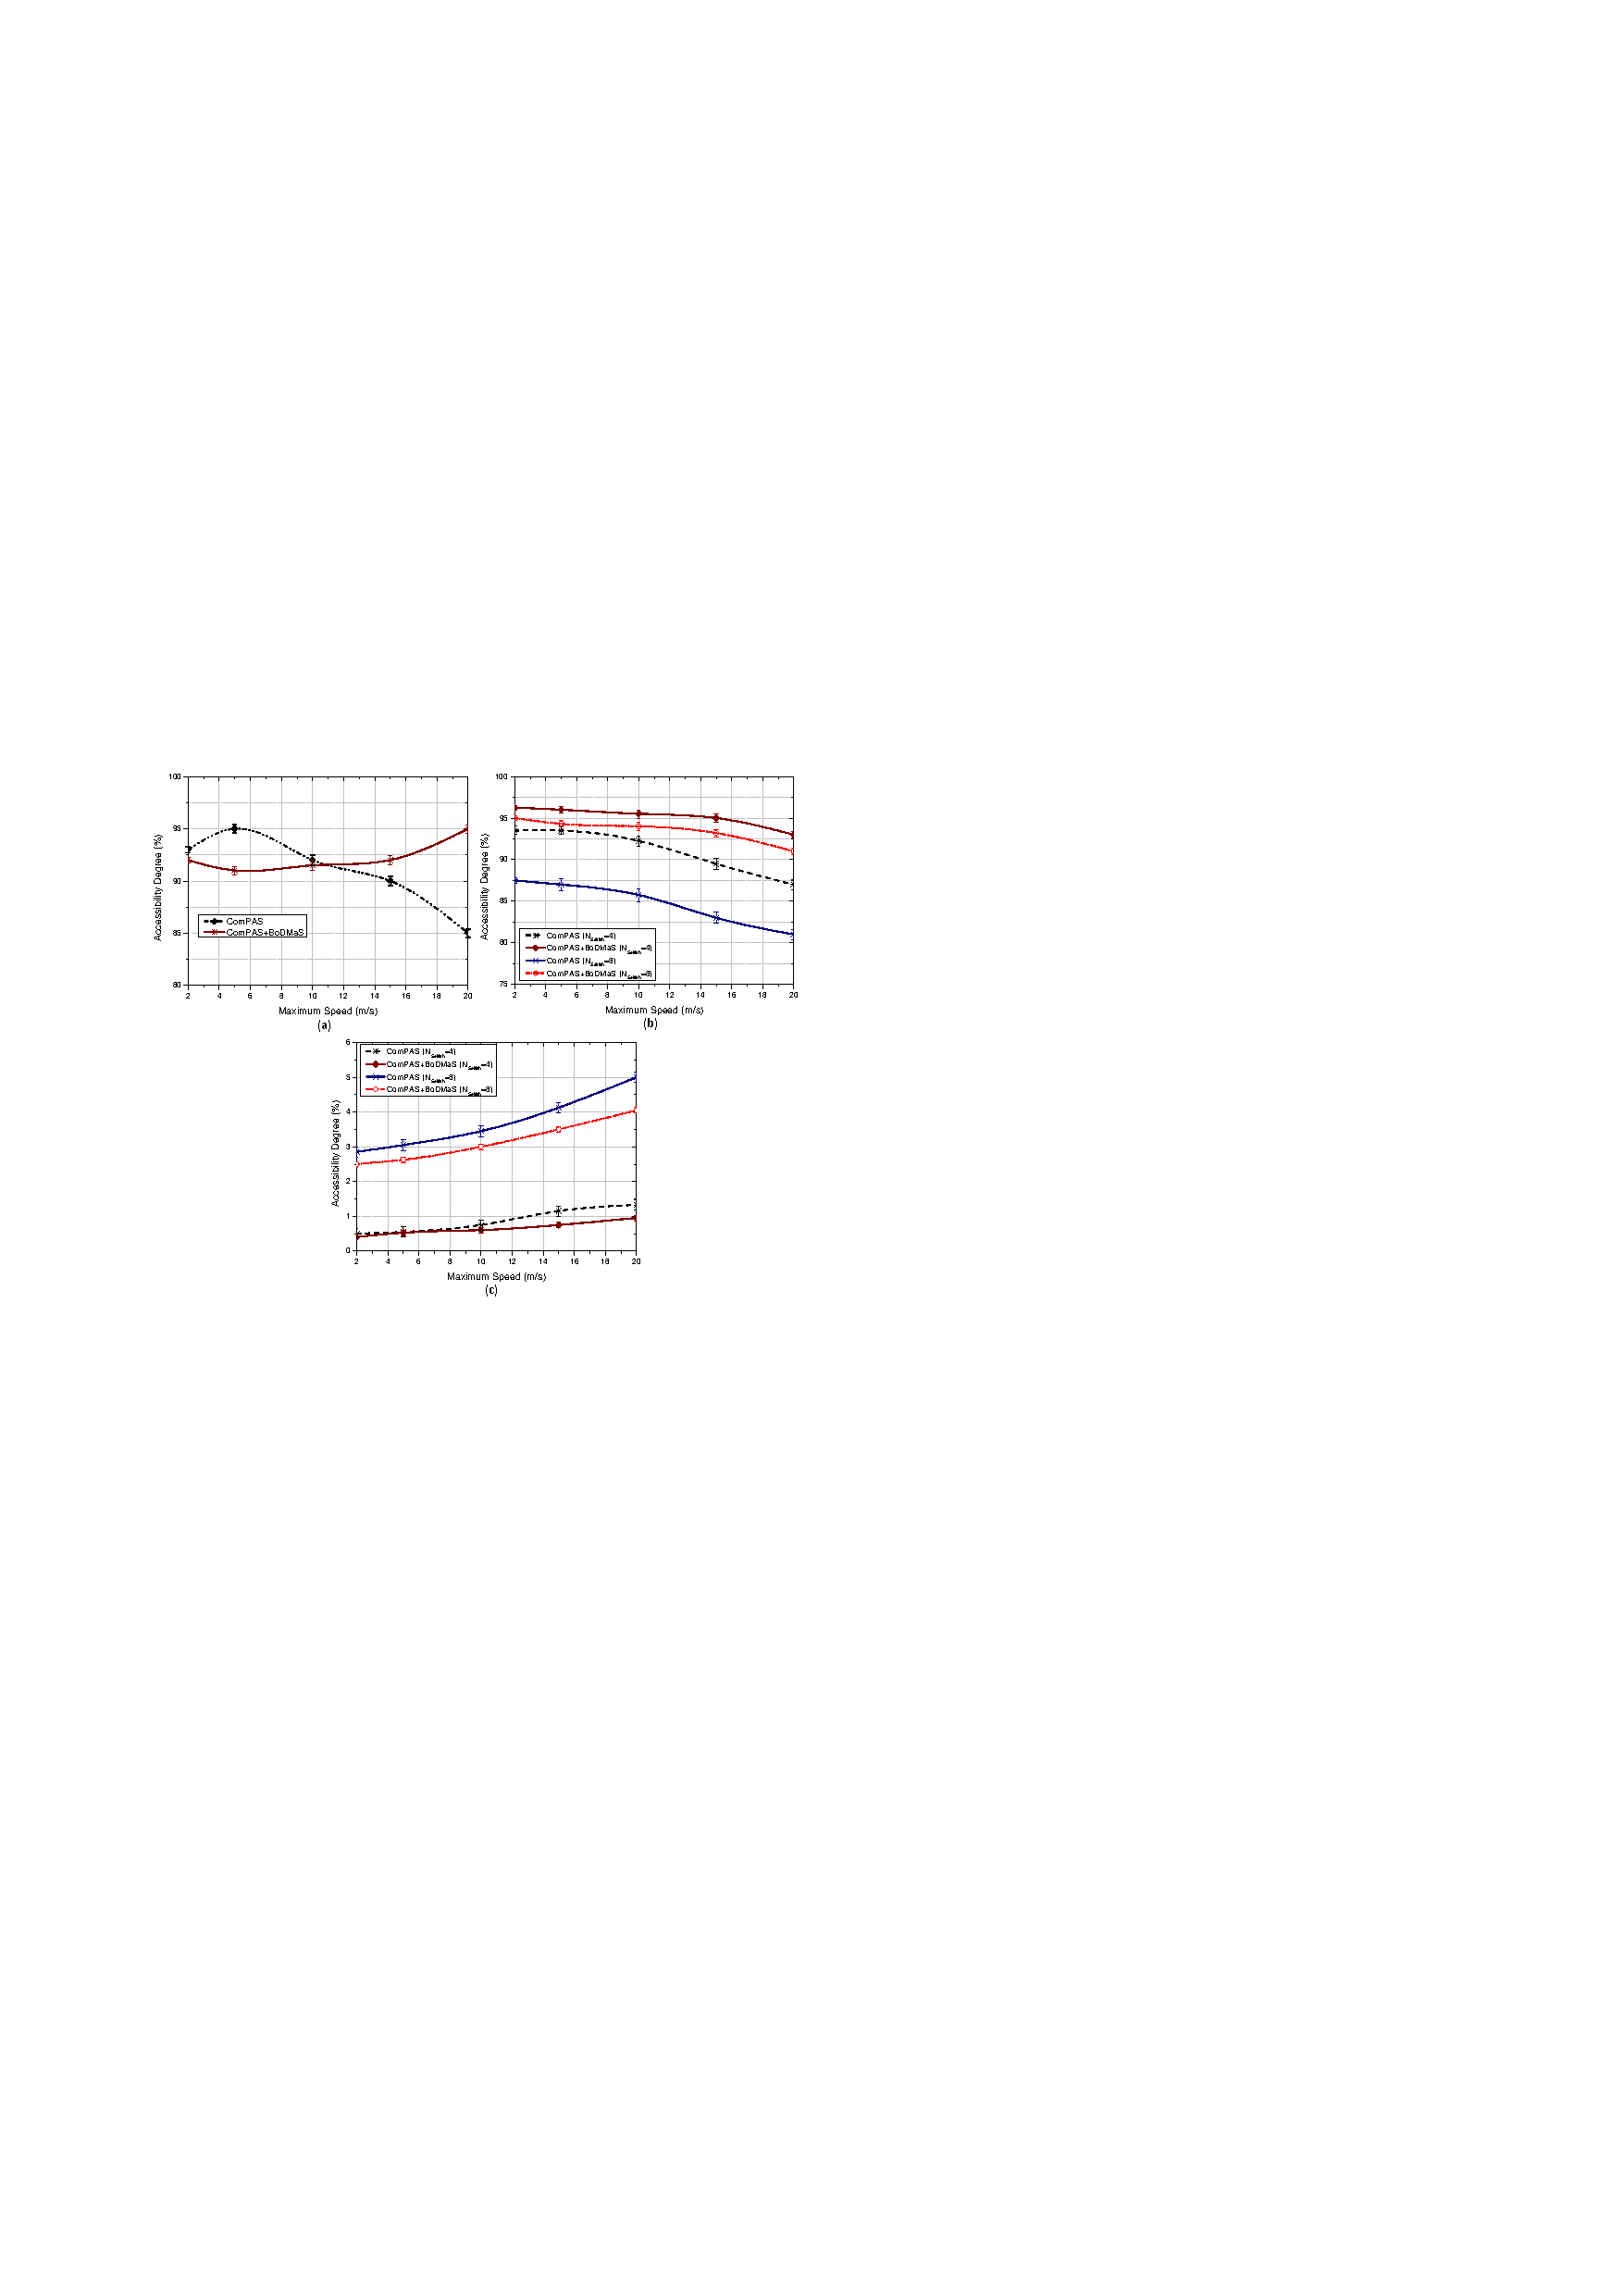
\includegraphics[width=0.95\textwidth]{Chap6-Fig6.pdf}
  \end{tabular}
  \caption{Accessibility degree for ComPAS$\uplus$BoDMaS and ComPAS; (a) without selfish users participation, and (b) with selfish users participation ($N_{Selfish}$ = 4 and $N_{Selfish}$ = 8) in update operations, (c) with selfish users participation ($N_{Selfish}$ = 4 and $N_{Selfish}$ = 8) in query operations.}
\end{center}
\end{figure}

Accessibility degree is the ratio of the number of successful access (query) requests to the number of all access requests issued which is an important metric for replication and reliability protocols. A replication method aims to increase the accessibility of data items in the network. Different from conventional static networks, in ASNETs achieving 100\% accessibility degree is nearly impossible due to mobility of nodes and changing network topology. To demonstrate effectiveness of integrated ComPAS and BoDMaS (ComPAS$\uplus$BoDMaS), we run simulation in two modes  for accessibility degree; firstly simulation in the presence of selfish users and secondly, simulation in the absence of selfish users. The results of our performance evaluation are depicted in Fig. 6.6.

Results of accessibility degree in the absence of selfish users for both ComPAS and ComPAS$\uplus$BoDMaS are illustrated in Fig. 6.6(a) when maximum speed increases from 2 to 10 m/s.  In low speed from 2 to 15 m/s, ComPAS$\uplus$BoDMaS does not shows positive accessibility improvement. However, as the maximum speed grows to 20 m/s, the difference is higher (from 85\% to 95\% for ComPAS and ComPAS$\uplus$BoDMaS, respectively). Evaluation results advocate that the proposed scheme shows a better performance than ComPAS in high speed mobilities, because, distant BoDMaS users (from other users) and those with smaller social willingness (connectivity) are not chosen to participate in the replica query and update operations. This also shows that the proposed scheme enforces a minimal trade-off between accessibility and security.

As displayed in Fig. 6.6(b), the use of BoDMaS shows an average improvement of 4.31\% and 8.94\% compared to the accessibility degree obtained by ComPAS without using BoDMaS in update operations for selfish users' participation with 4 and 8 respectively. The numbers of participating selfish users and the maximum speed have visible influence in ComPAS$\uplus$BoDMaS for both operations (Figs. 6.6(b) and (c)), when compared to ComPAS. However, as depicted in Fig. 6.6(c), with low variation, the evaluation presents lower results than ComPAS for query operations. This is because effect of selfishness for accessibility degree is less on query operations as compared to update operations. In the remaining part of this section, we focus on demonstrating the effectiveness of the proposed scheme in terms of true and false detection rates for query and update operations as well as network load balance.

\subsection{Detection Rate}\label{Chap6_05_02}
\esubsection{Detection Rate}
Detection rates obtained by BoDMaS for selfish user in query and update operations are illustrated in Figs. 6.7(a)-(c) and 6.8(a)-(c), respectively. TDR for query and update operations are presented in Figs. 6.7(a) and 6.8(a), while FDR (FN and FP) for query and update operations are presented in Figs. 6.7(b) \& (c) and 6.8(b) \& (c), respectively.

\subsubsection{Query Operation}\label{Chap6_05_02_01}
%\esubsubsection{Query Operation}
As depicted in Fig. 6.7(a), number of selfish users have visible impacts on detection rate results. For instance,  with 2 selfish users ($N_{Selfish}$ = 2) at a maximum speed of 2m/s, 5m/s, 10m/s, 15m/s and 20 m/s, the true detection rate for query operation is around 95.5\%, 95.6\%, 96\%, 95.8\% and 95.35\%, respectively. With 16 selfish users' participation ($N_{selfish}$ = 16) at a maximum speed of 2m/s, 5m/s, 10m/s, 15m/s and 20 m/s, the true detection rate for query operation is around 92.25\%, 92.5\%, 92.1\%, 91.625\% and 91\%, respectively. However, the TDR of selfish users in query operation for all the cases is higher than 90.95\%, because the proposed algorithm continuously assesses the selfish behavior of users and changes its status from selfish to cooperative when user resumes collaboration in forwarding query operations. Fig. 6.7(b) displays 1.2\% lower FN detection rate which shows very small error rate in mistakenly classifying selfish users as cooperative. This is due to the BoDMaS feature that counts $A_i$, individually. Furthermore, we evaluate FP detection rate as shown in Fig. 6.7(c) which is also a relatively small rate in mistakenly detecting cooperative users as selfish.
\begin{figure}[t]
\begin{center}
  \begin{tabular}{c}
  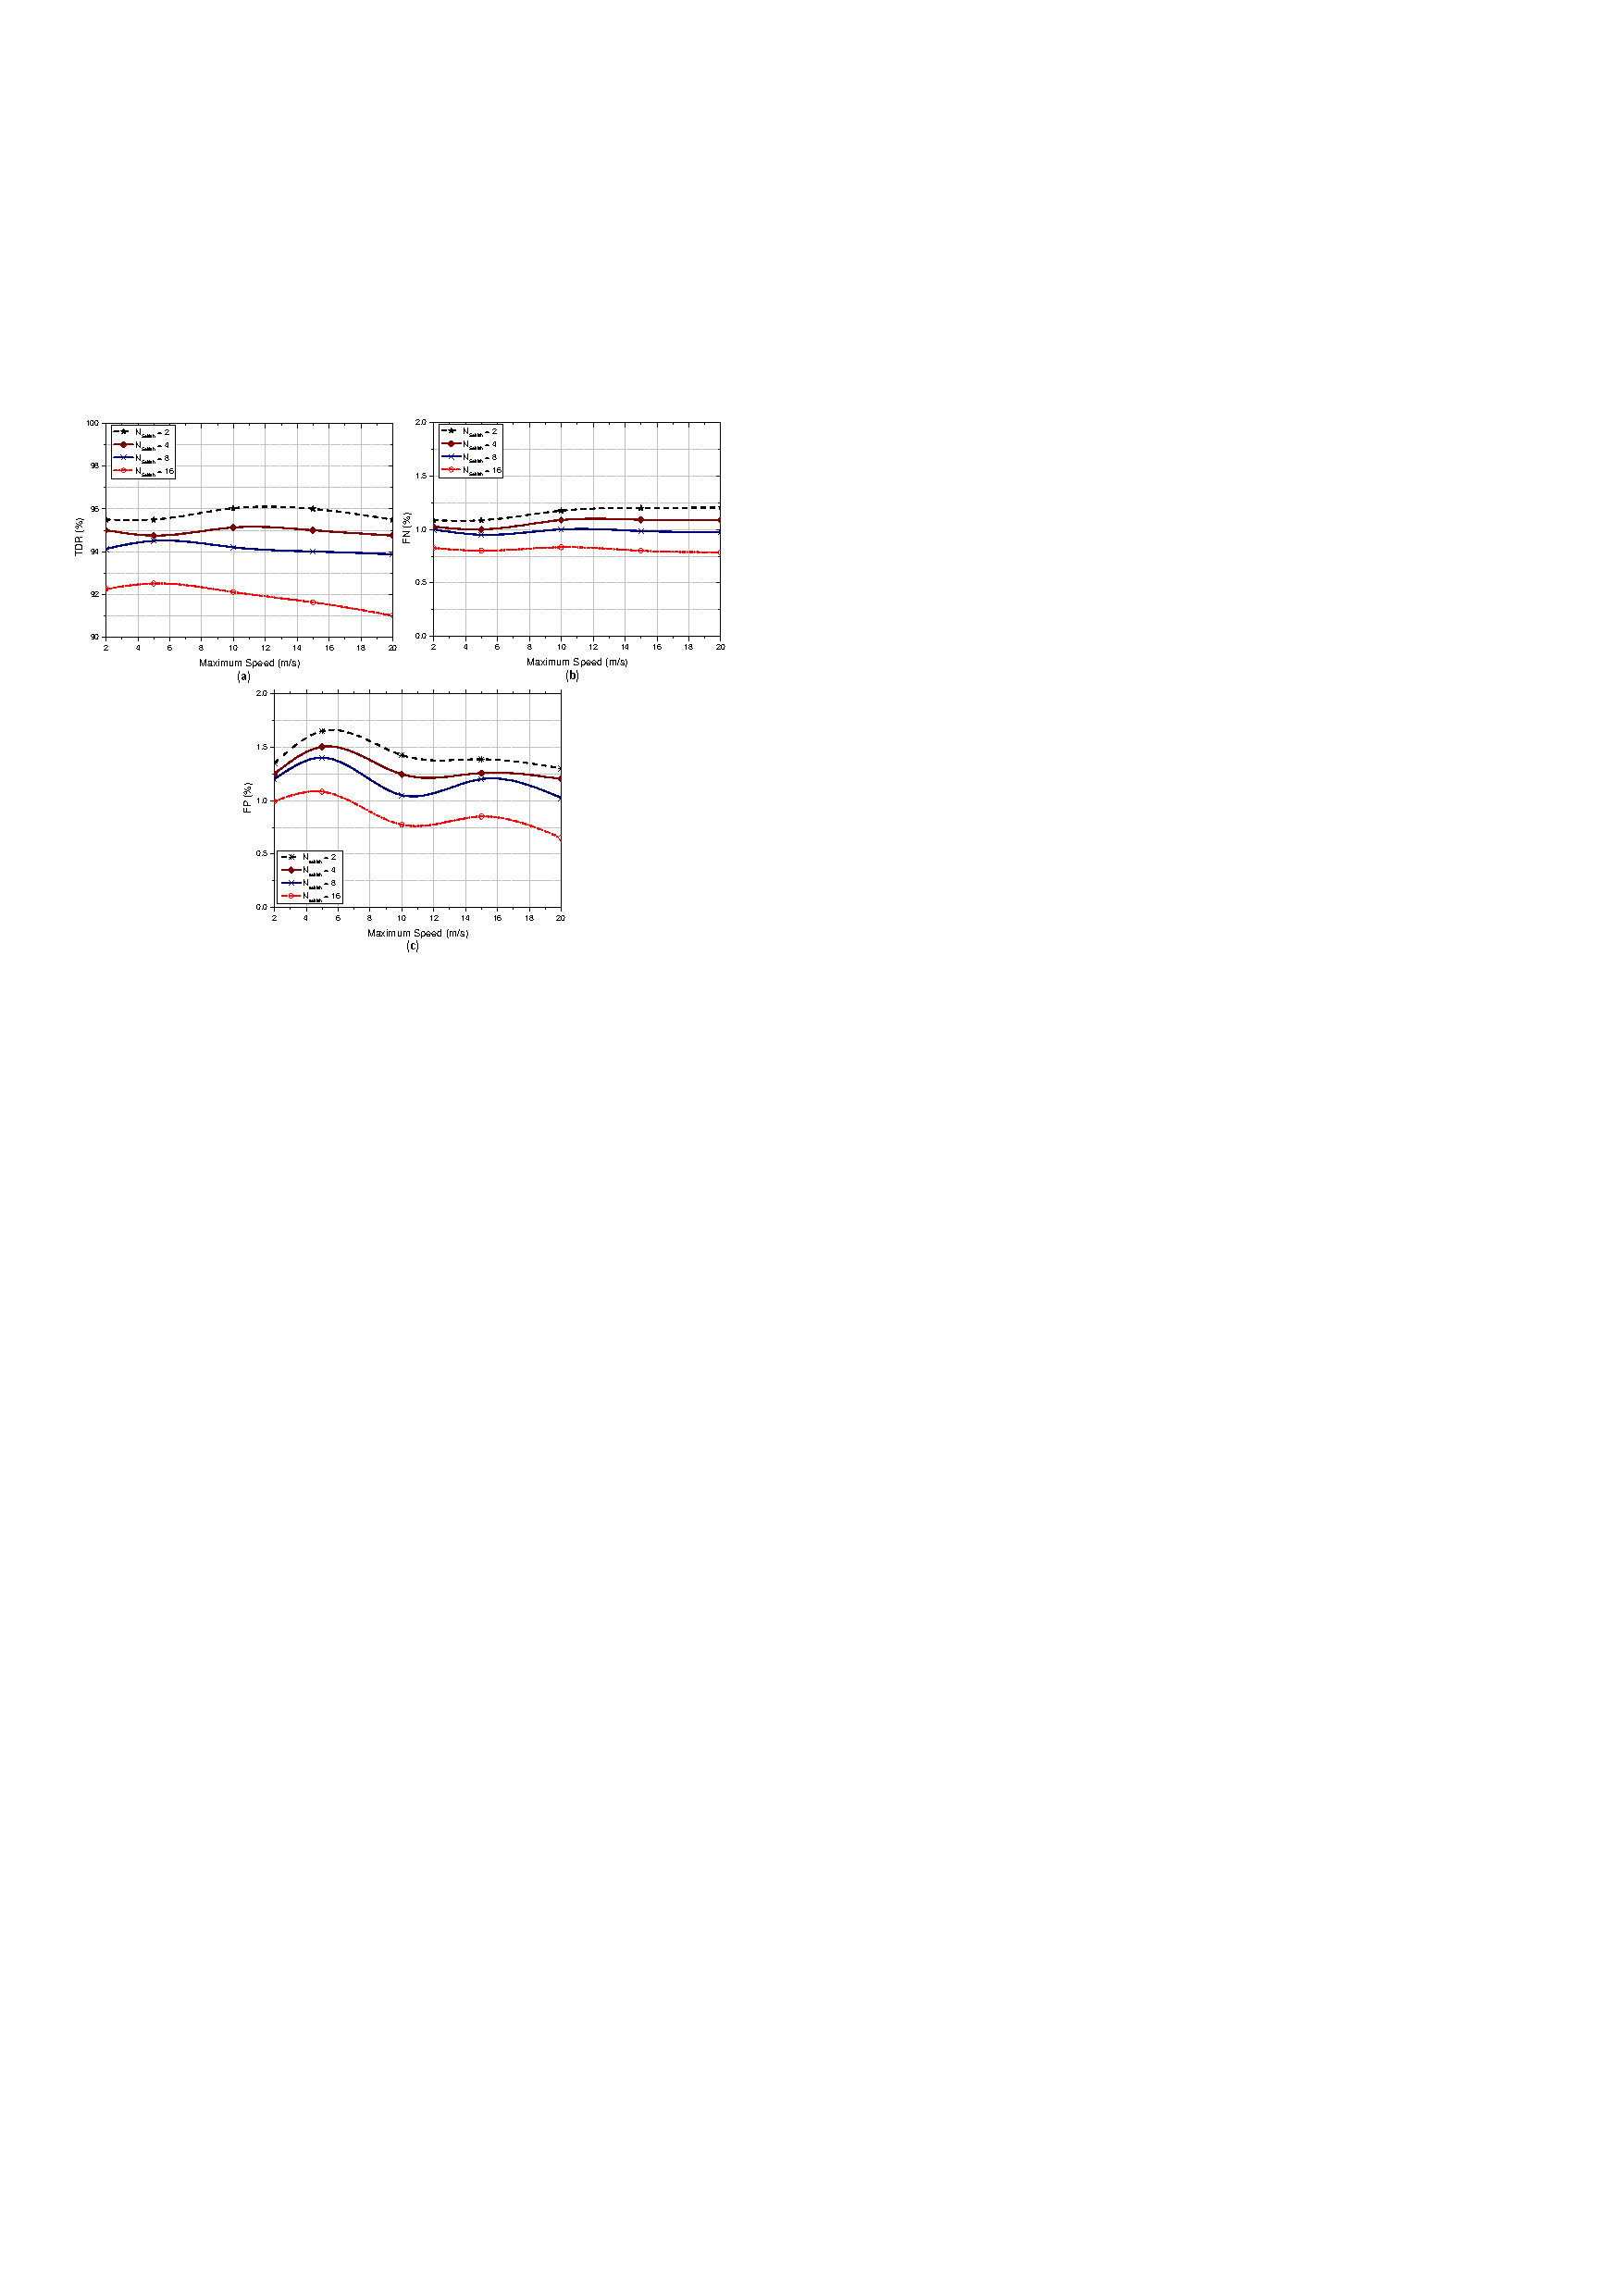
\includegraphics[width=0.95\textwidth]{Chap6-Fig7.pdf}
  \end{tabular}
  \caption{BoDMaS detection rate of selfishness in query operations; (a) true detection rate (TDR), (b) false negative (FN), and (c) false positive (FP).}
\end{center}
\end{figure}

\subsubsection{Update Operation}\label{Chap6_05_02_02}
%\esubsubsection{Update Operation}
\begin{figure}[t]
\begin{center}
  \begin{tabular}{c}
  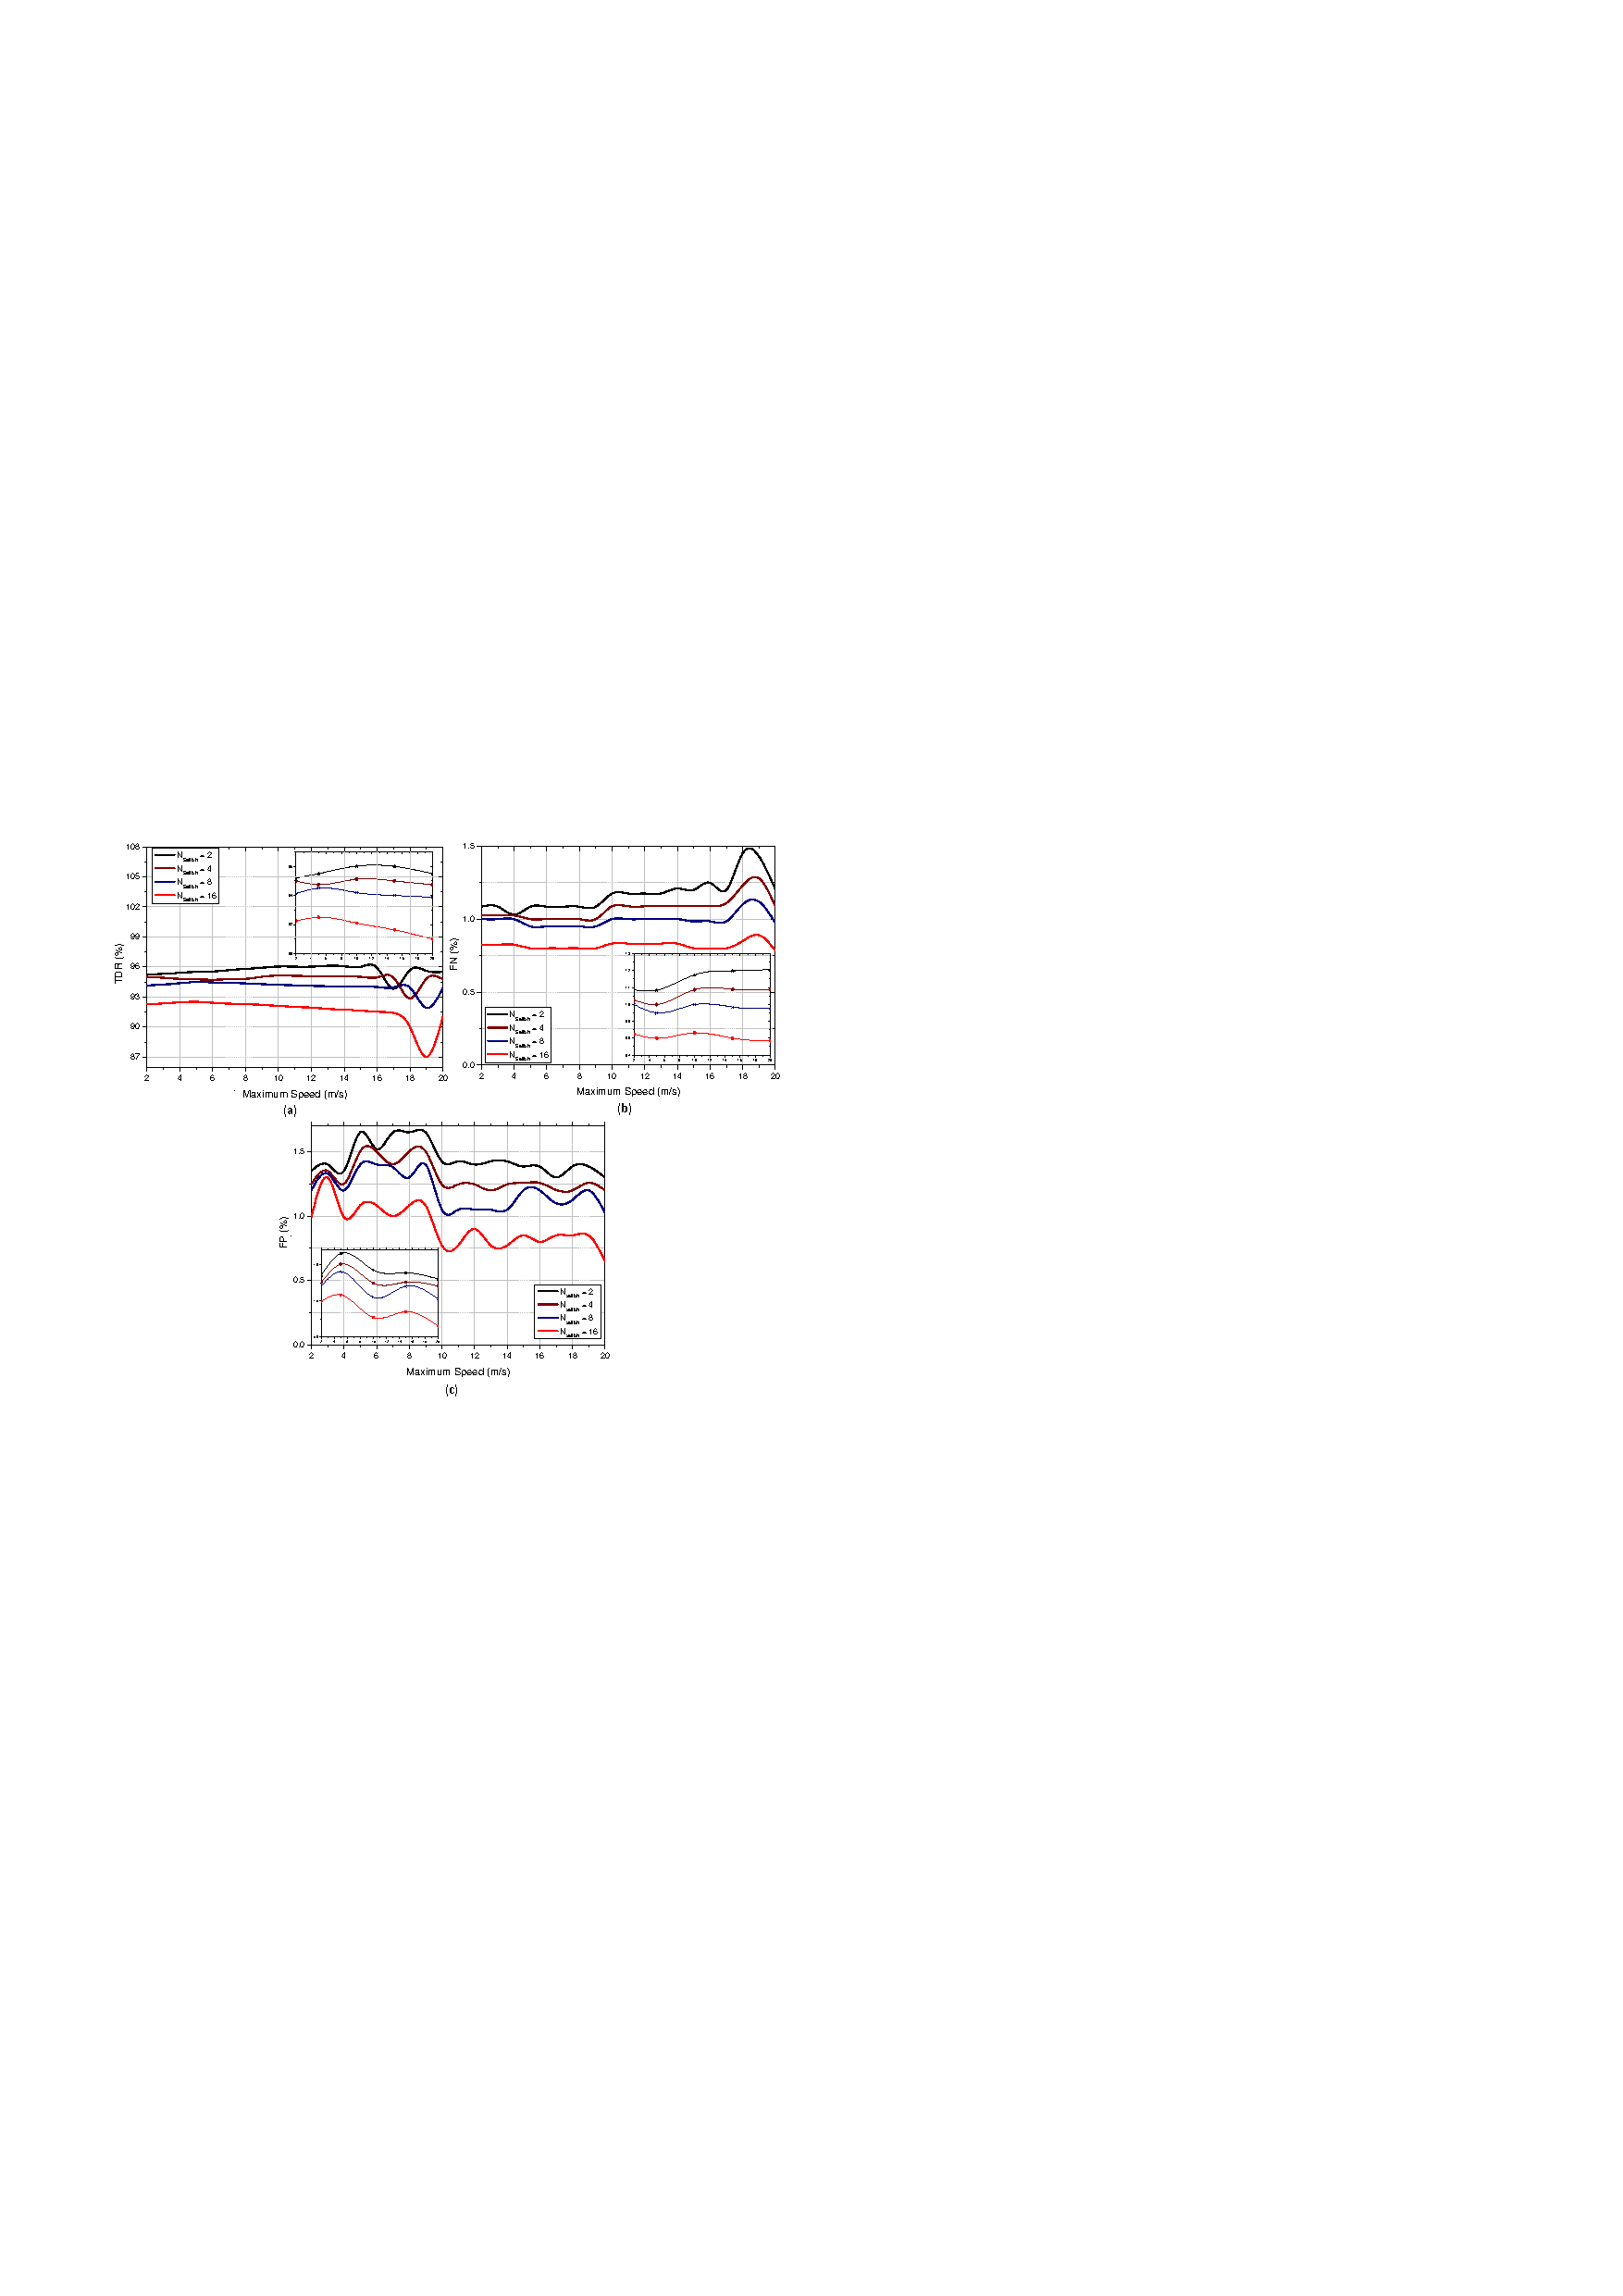
\includegraphics[width=0.95\textwidth]{Chap6-Fig8.pdf}
  \end{tabular}
  \caption{BoDMaS detection rate of selfishness in update operations; (a) true detection rate (TDR), (b) false negative (FN), and (c) false positive (FP).}
\end{center}
\end{figure}
In order to evaluate the efficiency of BoDMaS during update operation, we simulated operation in varied scenarios with different numbers of selfish users ($N_{Selfish}$ = 2, 4, 8 and 16) and analyzed detection rates (i.e., TDR and FDR). Results of our simulation are presented in two ways as shown in Figs. 6.8(a)-(c).  The detection rates with 2m/s, 5m/s, 10m/s, 15m/s and 20m/s on update operations are very similar to query operation. We depict them as small charts inside each chart in Fig. 6.8.
Therefore, we suspected how the result shows similarity for these two different operations while there are some users which might be malicious to be considered as selfish due to the timeout manipulation on the data.

Timeout manipulation is considered in our scheme and it is experienced in update operations only. In order to verify this, we run the scheme with participation of 2, 4, 8 and 16 selfish users' for continuous maximum speeds in a range of 2m/s and 20m/s. For all the detection rates this behavior (existence of timeout manipulation on update operation) proved to be true, as seen in Figs. 6.8(a)-(c). While TDR is higher than 90\% for almost all cases, there is a point where this rate goes down below 90\% with a speed of around 18m/s as shown in Fig. 6.8(a). This is because some users are not considered as selfish, but have the behavior of malicious users happen partly as a timeout manipulation. The same is repeated for false negative and false positive detection rates as depicted in Figs. 6.8(b) and (c), respectively. This is an evidence to consider and improve the consistency of our scheme in terms of detection rates for update operations. Moreover, BoDMaS obtained good detection rates for update operations with the specified maximum mobility of users in the scenario.

\subsection{Network Load Balance}\label{Chap6_05_03}
\esubsection{Network Load Balance}
\begin{figure}[t]
\begin{center}
  \begin{tabular}{c}
  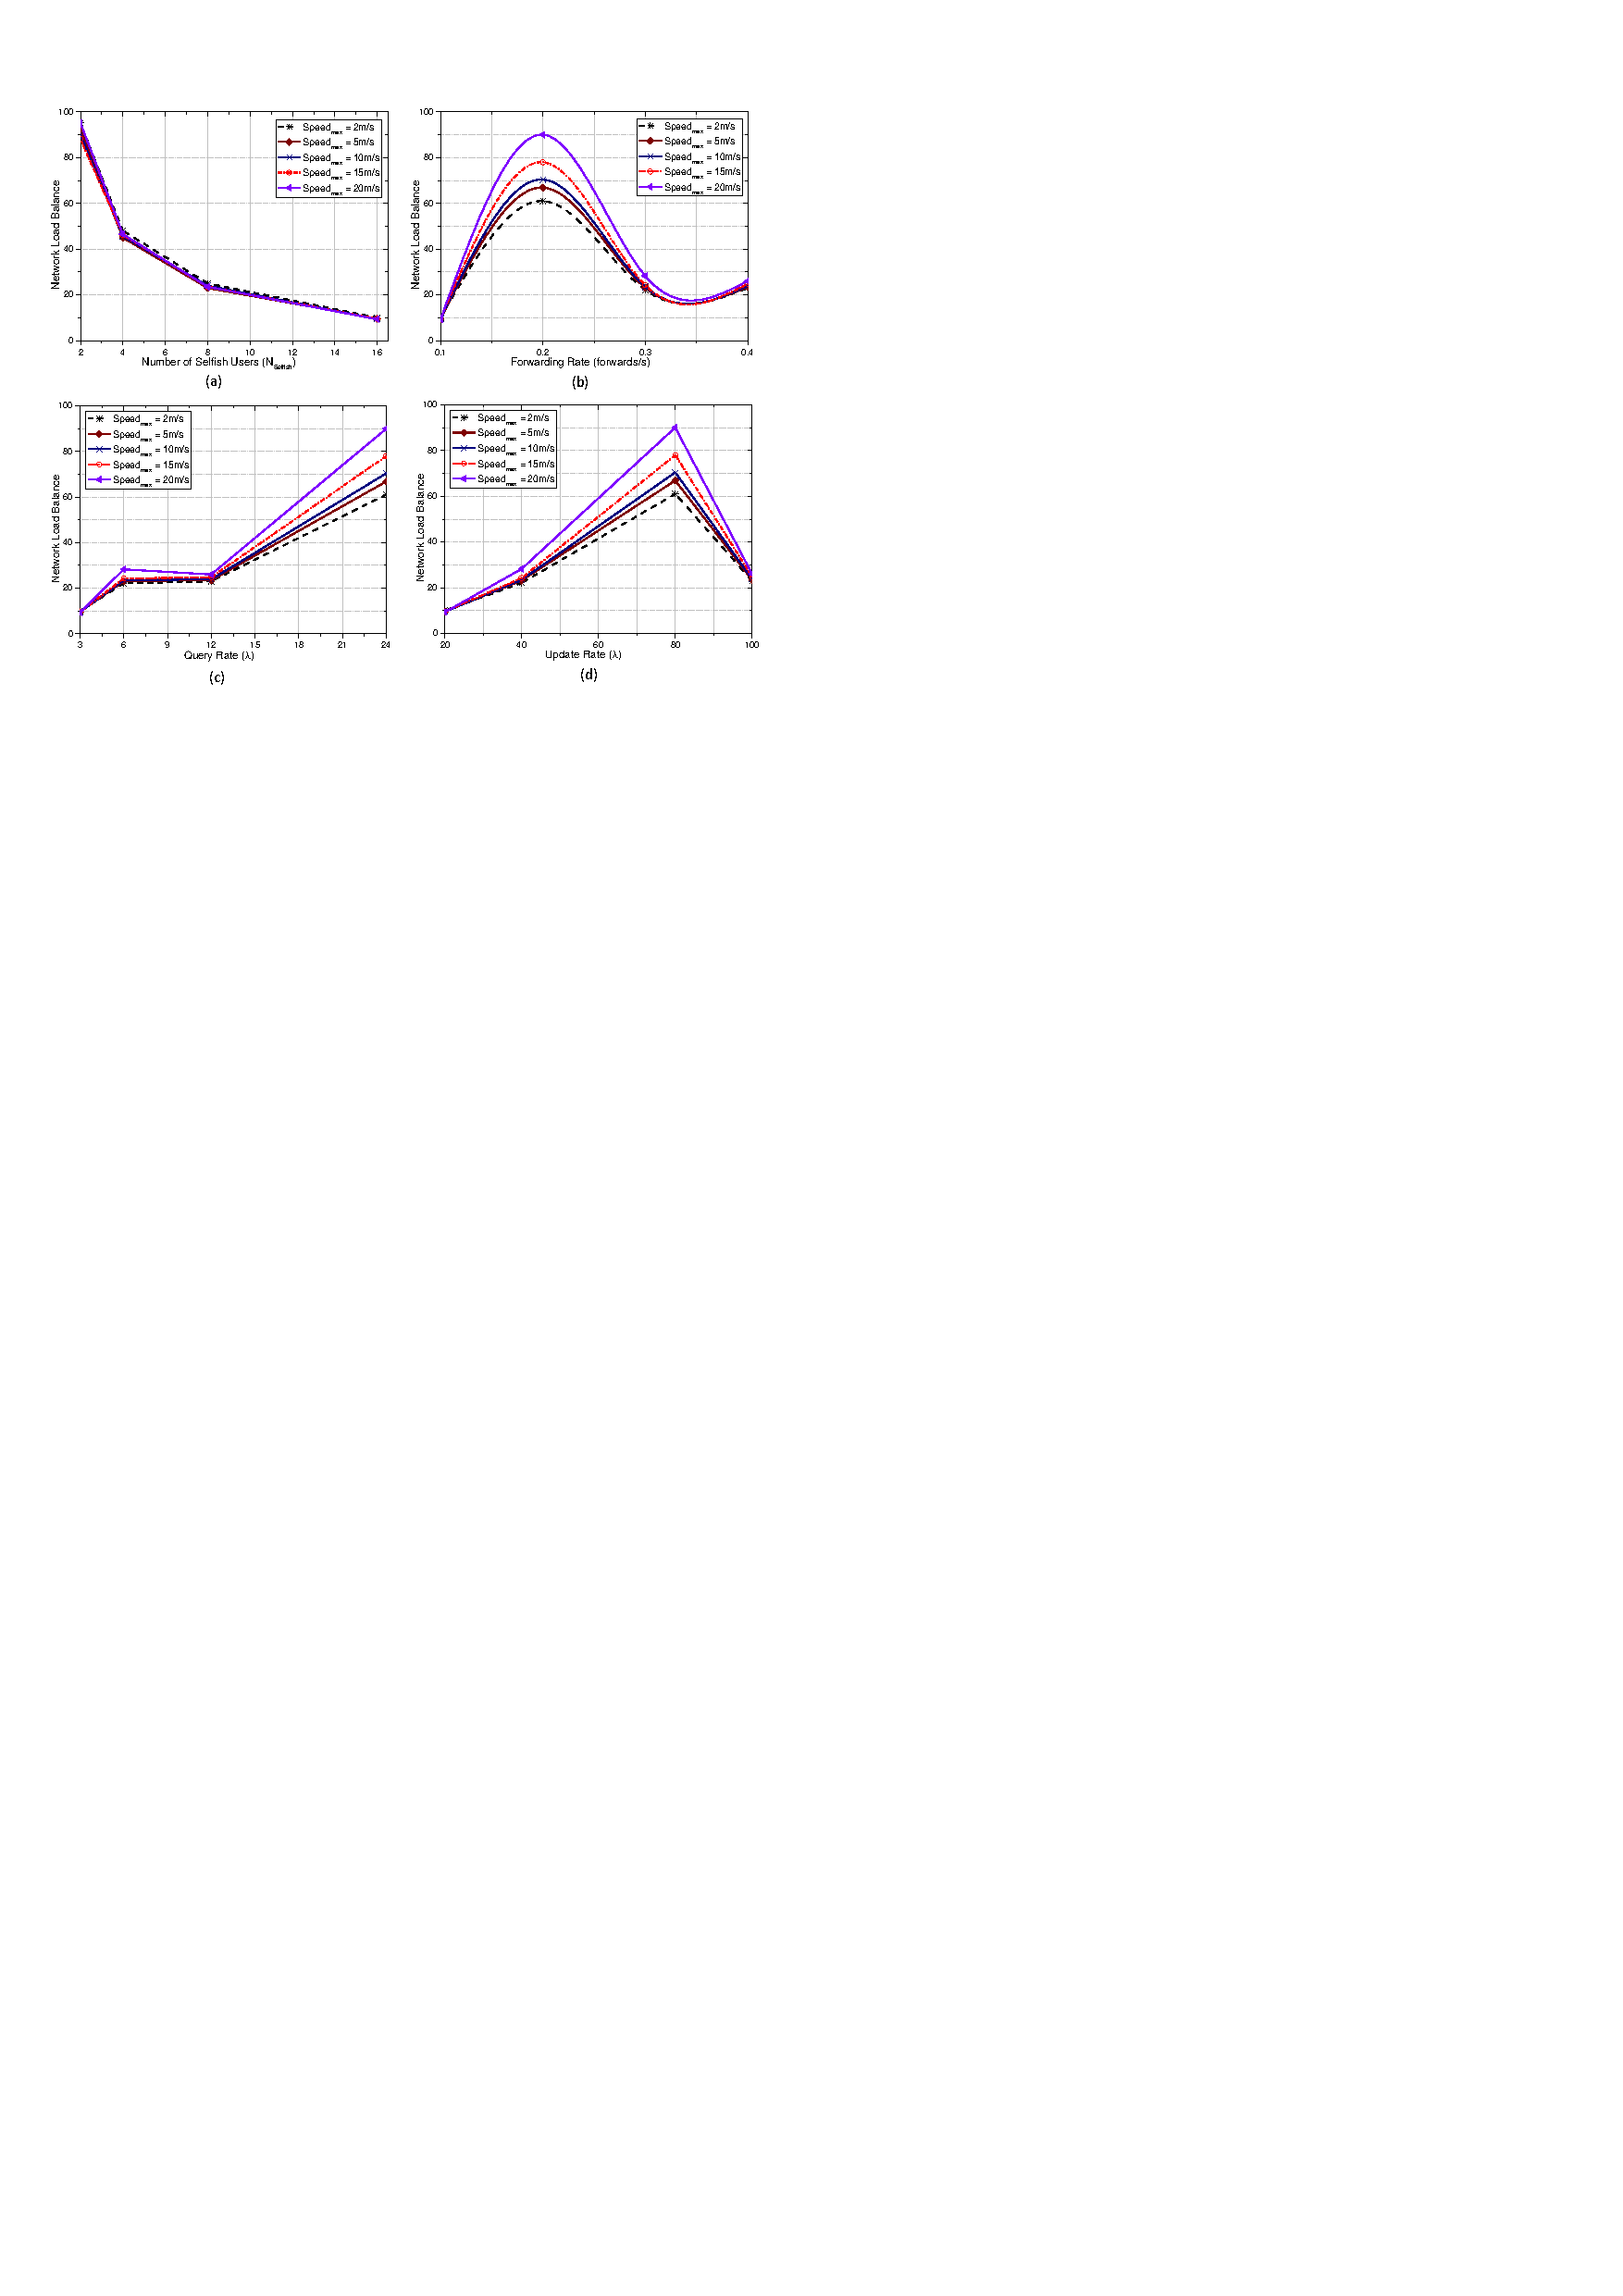
\includegraphics[width=0.9\textwidth]{Chap6-Fig9.pdf}
  \end{tabular}
  \caption{BoDMaS network load balance efficiency in terms of; (a) number of selfish users ($N_{Selfish}$), (b) forwarding rate, (c) query rate, and (d) update rate.}
\end{center}
\end{figure}

Network load balance is the ability of our algorithm to balance traffic across users (including the operations) of network scenario without applying load balancing and fairness mechanisms. The evaluations of network load balance are presented in four ways as shown in Figs. 6.9(a)-(d). The effect of number of selfish users on the network load balance is depicted in Fig. 6.9(a). The network load balance decreases from 90\% to 15\% with the increase in the numbers of selfish users participation (from $N_{Selfish} = 2$ to $N_{Selfish}=16$) due to resource wastage of selfish users. However, network load balance doesn't change when speed changes from 2m/s to 20m/s, which means that network load balance in BoDMaS is not much influenced by differences in low and high user mobility. The main reason for this anomaly is that the participation of selfish users has a dominating effect in most cases than the speed of these users. As described at the very beginning of this section, we set threshold values for forwarding, query, and update rates. Using Figs. 6.9(b)-(d), we demonstrate the probability that how our choices of the values are comparably successful based on the network load balance even if we only compare with very few values. Based on these observations, the ability of our algorithm to balance traffic across users is successful using the threshold values; forward threshold of 0.2, query rate of 24 and update rate of 80 as shown in Fig. 6.9(b), Fig. 6.9(c) and Fig. 6.9(d), respectively. Moreover, unlike Fig. 6.9(a), the network load balance shows an increasing behavior when the mobility of users (speed) is higher.

Overall, according to the simulation results shown in Figs. 6.6 - 6.9, we have demonstrated the effectiveness of our algorithm in terms of accessibility degree, detection rates (true detection rate and false detection rate) and network load balance.

\section{Summary}\label{Chap6_06}
\esection{Summary}
In this chapter, we have demonstrated the feasibility and significance of integrating social willingness with quorum sensing (a well-known bio-inspired mechanisms) to detect and counteract selfishness in ASNET. We introduced BoDMaS, an algorithm that assesses user's social tie with quorum sensing to classify users as either selfish or cooperative. BoDMaS exploits user classification results to inhibit selfish users from performing operation in network and also alert cooperative users to stop forwarding requests to selfish users. For effective evaluation of BoDMaS, we integrate it with ComPAS (a socially-aware replication system that ensures high availability in ASNETs, as proposed in chapter \ref{chap02}) and run series of simulations in an academic conference and analyzed three metrics, namely accessibility degree, detection rates, and network load balance. The evaluation results yield high TDR, low FN and FP with fast detection speed leading to enhanced data replication in ASNETs which are evidences of BoDMaS effectiveness. Moreover, BoDMaS is efficient in terms of the ability to balance traffic in varied network scenarios.
